% This is samplepaper.tex, a sample chapter demonstrating the
% LLNCS macro package for Springer Computer Science proceedings;
% Version 2.20 of 2017/10/04
%
\documentclass[runningheads]{llncs}
%\pagestyle{plain}
%
\usepackage{graphicx}
% Used for displaying a sample figure. If possible, figure files should
% be included in EPS format.
%
% If you use the hyperref package, please uncomment the following line
% to display URLs in blue roman font according to Springer's eBook style:
% \renewcommand\UrlFont{\color{blue}\rmfamily}

\usepackage{amssymb}
\usepackage[super]{nth}

\usepackage{algorithm}
\usepackage{algorithmicx}
\usepackage{algpseudocode}
\usepackage{multirow}
\usepackage{amsmath}
\usepackage{extarrows}
\usepackage{pgf}
%\usepackage{subfig}
\usepackage{subfigure}

\newif\ifsans
\newif\iftext
\newif\ifdetails
\usepackage{tikz}
\tikzset{sparsam/.style={inner sep=1pt}}
\tikzset{bitwidth/.style={above=-1pt, font=\tiny}}
\tikzset{next/.style={->, >=latex}}
\usetikzlibrary{crypto.symbols,decorations.pathreplacing}
%\usetikzlibrary{arrows,shapes,snakes,automata,backgrounds,petri}

%usepackage{algpseudocode}
%\algdef{SE}[DOWHILE]{Do}{doWhile}{\algorithmicdo}[1]{\algorithmicwhile\ #1}%

\renewcommand{\algorithmicrequire}{\textbf{Input:}}
\renewcommand{\algorithmicensure}{\textbf{Output:}}

\newcommand{\ith}{i\textsuperscript{th} }
\newcommand{\Prob}{\text{Prob}}
\newcommand{\Cor}{\text{Cor}}
\newcommand{\EDP}{\text{EDP}}
\newcommand{\ELP}{\text{ELP}}
\newcommand{\Exp}{\text{Exp}}
\newcommand{\calE}{\mathcal{E}}
\newcommand{\calP}{\mathcal{P}}
\newcommand{\calH}{\mathcal{H}}
\newcommand{\calR}{\mathcal{R}}
\newcommand{\calA}{\mathcal{A}}
\newcommand{\calS}{\mathcal{S}}
\newcommand{\calL}{\mathcal{L}}
\newcommand{\calO}{\mathcal{O}}
\newcommand{\bbF}{\mathbb{F}}
\newcommand{\bbP}{\mathbb{P}}
\newcommand{\true}{\text{true}}
\newcommand{\false}{\text{false}}
\newcommand{\rotr}{\text{rotr}}
\newcommand{\rotl}{\text{rotl}}
\newcommand{\Asn}{\text{Asn}}
\makeatletter
\newenvironment{breakablealgorithm}
  {% \begin{breakablealgorithm}
   \begin{center}
     \refstepcounter{algorithm}% New algorithm
     \hrule height.8pt depth0pt \kern2pt% \@fs@pre for \@fs@ruled
     \renewcommand{\caption}[2][\relax]{% Make a new \caption
       {\raggedright\textbf{\ALG@name~\thealgorithm} ##2\par}%
       \ifx\relax##1\relax % #1 is \relax
         \addcontentsline{loa}{algorithm}{\protect\numberline{\thealgorithm}##2}%
       \else % #1 is not \relax
         \addcontentsline{loa}{algorithm}{\protect\numberline{\thealgorithm}##1}%
       \fi
       \kern2pt\hrule\kern2pt
     }
  }{% \end{breakablealgorithm}
     \kern2pt\hrule\relax% \@fs@post for \@fs@ruled
   \end{center}
  }
\makeatother

\begin{document}
%
\title{An Automatic Search Tool for Iterative Distinguishers and its Application to Finding Differentials and Linear Hulls
%\thanks{Supported by organization x.}
}
%
\titlerunning{An Automatic Search Tool for Iterative Distinguishers}
% If the paper title is too long for the running head, you can set
% an abbreviated paper title here
%
%\author{Tianyou Ding\inst{1,2}
%\orcidID{0000-1111-2222-3333} 
%\and Wentao Zhang\inst{1,2}
%\and Chunning Zhou\inst{1,2}
%\and Fulei Ji\inst{1,2}
%}
%
%\authorrunning{Tianyou Ding et al.}
% First names are abbreviated in the running head.
% If there are more than two authors, 'et al.' is used.
%
%\institute{State Key Laboratory of Information Security, Institute of Information Engineering, Chinese Academy of Sciences, Beijing, China\\
%\email{\{dingtianyou, zhangwentao, zhouchunning, jifulei\}@iie.ac.cn}
%\and School of Cyber Security, University of Chinese Academy of Sciences, Beijing, China
%}
%
\maketitle              % typeset the header of the contribution
%
\begin{abstract}

%The design and cryptanalysis are the both sides from which we look at symmetric-key primitives. If a symmetric-key primitive is broken by a kind of cryptanalysis, it's definitely insecure. If a designer claims a symmetric-key primitive to be secure, one should demonstrate that the primitive resists against all known attacks. 

Differential and linear cryptanalysis are two of the most important kinds of cryptanalysis for symmetric-key primitives. To conduct a successful differential (linear) cryptanalysis, a differential (linear) distinguisher with high differential probability (correlation amplitude) is needed. 

In this paper, we propose our method of searching for iterative differential and linear distinguishers for SPN symmetric-key primitives using a graph approach. We further propose our method of searching for the best differential or linear hull containing iteractive sub-characteristics. 

We apply our methods to 6 SPN symmetric-key primitives. For KNOT, PUFFIN and TRIFLE, we find better differential and linear distinguishers. For KNOT, we mount different round-reduced attacks according to the different phases targetted and show that KNOT has enough security margin against differential and linear cryptanalysis considering the clustering effect. What's more, by visualizing the graph composed of iteractive characteristics, we hope to shed some light on the design of lightweight SPN symmetric-key primitives. 

%Comparing results considering single characteristics and results considering the clustering effect

%We find that iterative characteristics can always be found for them. By considering the clustering effect, we find better iterative distinguishers. Using the knowledge of iterative characteristics, we estimate EDPs and ELPs. By comparison with results using other methods, we illustrate that the assumption of the dominance of iterative characteristics is reasonable. 


%%For some lightweight symmetric-key primitives, their best trails contain iterative trails. In this work, We present an algorithm searching for iterative trails by modelling it into a graph problem. We find that the clustering effect of iterative trails may enhance differential and linear propagations. If iterative trails found, we propose a method to estimate the probability (correlation) of differentials (linear hulls). 

%%We apply our methods to 256-bit KNOT permutation, ASCON permutation, PRESENT, GIFT-64 and RECTANGLE. The found iterative trails form a directed graph and are visualized. If iterative trails are found, our method can efficiently find good differentials and linear hulls. Our results imply that for the primitives we experiment on with bit permutations as their linear layers, the best differentials and linear hulls are dominated by iterative trails. 

%%For KNOT, which is a round 2 candidate of the NIST lightweight cryptography standardization process, we find differential and linear distinguishers with certain restrictions and truncations on the input and output differences or masks, which adapt the distinguishers to certain differential or linear attacks on the AEAD and Hash schemes. 

%An upper bound of the weight of the best trail with arbitrary rounds is obtained in several seconds. When the number of rounds is large, it's illustrated that the upper bound coincide with the best weight or is very tight. An upper bound of the weight of the best differential or linear propagation is also obtained by considering the clustering effect. For 14-round 256-bit KNOT permutation, 13-round GIFT-64 and 15-round RECTANGLE, better differential distinguishers than the best differential trails are obtained. For 10-round 256-bit KNOT permutation and 13-round RECTANGLE, better linear distinguishers than the best linear trails are obtained. Additionally, by constraining the input and output differences and masks, results for KNOT-AEAD fitting certain differential and linear attack scenarios in Duplex mode of operations are obtained. 

\keywords{Differential cryptanalysis \and Linear cryptanalysis \and Iterative characteristics \and Graph theory \and Differentials \and Linear hulls}
\end{abstract}

\section{Introduction}

Differential cryptanalysis (DC) \cite{BS91,BS92} and linear cryptanalysis (LC) \cite{M93,M94_1} are two of the most powerful attacks against modern block ciphers. In 1990, Biham and Shamir introduced differential cryptanalysis and successfully attacked the full-round DES\cite{BS92}. In 1991, they improved the attack with $2^{47}$ chosen plaintexts\cite{BS92}. In 1993, Matsui introduced linear cryptanalysis and succeeded in breaking DES with $2^{47}$ known plaintexts\cite{M93}. In 1994, Matsui improved the data complexity to $2^{43}$\cite{M94_1}. Cryptanalysis also drives the design of ciphers in return. In 2001, Rijmen and Daemon proposed the wide trail design strategy\cite{DR01}, providing provable security against DC and LC for AES winner Rijndael\cite{DR98}. With increasing number of symmetric cryptographic primitives emerging, every well-designed block cipher must resist against DC and LC in the first place. To conduct the differential or linear attack, an adversary expects to find exploitable differential or linear distinguishers. Usually, the probability of the best differential trail and the correlation (or bias) of the best linear trail are respectively used as the indices to the resistance against DC and LC. The two main kinds of the automatic search tools for the best differential and linear trails are dedicated tree search algorithms \cite{M94_2,OMA95,AKM97,BZL14} and mathematical-solver-based methods \cite{MWG12,SHW14-1,SHW14-2,ZZDX19}. In this article, we focus on the dedicated search algorithms. 

In 1994, Matsui proposed a branch-and-bound depth-first tree search algorithm for searching the best differential or linear trail of DES\cite{M94_2}. In 1995, Moriai et al. introduced the concept of search pattern to reduce unnecessary search candidates, which improves the performance of searching the best trail of FEAL\cite{OMA95}. In 1997, Aoki et al. further improved the performance by using a pre-search for impossible search patterns\cite{AKM97}. In 2014, Bao et al. proposed new strategies including starting from the narrowest point, concretizing and grouping search patterns and trailing in minimal changes order, achieving significant efficiency improvement on NOEKEON and Spongent\cite{BZL14}. Dobraunig et al. \cite{DEM15} proposed a stack-based depth-first search algorithm characterizing in guessing sbox by sbox or bit by bit instead of round by round in Matsui's algorithm. Hall-Andersen et al. \cite{HV18} modeled the trail search as a graph problem and managed to obtain results on clustering effect for many ciphers. 

%Another line of research is modelling the differential or linear propagation and solve the model using mathematical tools. In 2011, Wu et al. modeled block ciphers using integer programming\cite{WW11}. Works that modelling using mixed integer linear programming (MILP) include but not limited to \cite{MWG12}. Works that modelling using SAT/SMT include but not limited to []. Works that modelling using constraint programming (CP) include but not limited to [].
Besides automatically searching the best differential or linear trail, iterative trails are used to construct long-round significant trails in order to efficiently obtain exploitable trails for cryptanalysis. Iterative trails refer to trails that have the same input and output difference (or mask) and thus they can concatenate to themselves. Biham and Shamir used iterative differential characteristics to cryptanalyze DES with an arbitrary number of rounds\cite{BS91,BS92}. Knudsen examined the 2 iterative characteristics found in \cite{BS91,BS92} and found additional 3 iterative characteristics for DES\cite{K92}. Wang et al. found a 4-round iterative differential characteristic for PRESENT by which a 14-round significant differential characteristic is constructed\cite{W08}. 
%If the iterative structure is not too complicated, our method is able to find all iterative trails in seconds. Using the iterative structure, We can further determine the weight of the best $n$-round trails constructed by iterative trails. 

%\begin{table}
%	\caption{results on weights of best trails and clusters}\label{tab:sum}
%	\centering
%	\begin{tabular}{|c|c|c|c|c|c|}
%        \hline
%        cipher&target&round&best weight&method&time\\
%        \hline
%        \multirow{9}{*}{KNOT-perm-256}
%        &differential trail   &14     &71         &\cite{ZDY19}           &-\\
%        &differential cluster  &14     &$\leq$ 65.4493    &Sec. \ref{sec:para3}   &511s\\
%        &differential trail   &48     &252         &\cite{BZL14}           &2.87h\\
%        &differential trail   &48     &$\leq$ 252        &Sec. \ref{sec:para2}   &0.1s\\
%        \cline{2-6}
%        &linear trail         &10     &23         &\cite{ZDY19}            &-\\
%        &linear cluster        &10     &$\leq$ 21.8301    &Sec. \ref{sec:para3}   &7509s\\
%        &linear trail         &39     &110         &\cite{BZL14}            &344.01h\\
%        &linear trail         &39     &$\leq$ 110        &Sec. \ref{sec:para2}   &0.6s\\
%        &linear trail         &44     &$\leq$ 125        &Sec. \ref{sec:para2}   &0.6s\\
%        \hline
%        \multirow{4}{*}{PRESENT}
%        &differential trail   &14     &62         &\cite{ZZDX19}          &-\\
%        &differential trail   &14     &$\leq$ 62         &Sec. \ref{sec:para2}   &0.6s\\
%        \cline{2-6}
%        &linear trail     &16     &30         &\cite{ZZDX19}          &-\\
%        &linear trail      &16     &$\leq$ 30         &Sec. \ref{sec:para2}   &0.1s\\
%        \hline
%        \multirow{5}{*}{GIFT-64}
%        &differential trail   &13     &62         &\cite{ZZDX19}          &-\\
%        &differential trail   &13     &$\leq$ 62         &Sec. \ref{sec:para2}   &0.3s\\
%        &differential cluster   &13     &$\leq$ 60.415     &Sec. \ref{sec:para3}   &414s\\
%        \cline{2-6}
%        &linear trail         &12     &31         &\cite{ZZDX19}          &-\\
%        &linear trail         &12     &$\leq$ 32         &Sec. \ref{sec:para2}   &0.2s\\
%        \hline
%        \multirow{6}{*}{RECTANGLE}
%        &differential trail   &14     &61         &\cite{ZBL15}           &-\\
%        &differential trail   &14     &$\leq$ 61         &Sec. \ref{sec:para2}   &1.2s\\
%        &differential cluster   &15     &$\leq$ 63.7857    &Sec. \ref{sec:para3}   &1329s\\
%        \cline{2-6}
%        &linear trail         &13     &31         &\cite{ZBL15}            &-\\
%        &linear trail         &13     &$\leq$ 31         &Sec. \ref{sec:para2}   &0.2s\\
%        &linear cluster ($c^2$)  &13     &$\leq$ 59.3561    &Sec. \ref{sec:para3}   &2481s\\
%        \hline
%	\end{tabular}
%\end{table}

\subsubsection{Our Contribution}
%\begin{enumerate}
%    \item We propose a new automatic tool for searching iterative trails for permutations or block ciphers based on S-boxes. We introduce the concept of $k$-hinge trails by which a directed graph is formed. Inspired by Johnson's algorithm \cite{J75} of finding all the elementary circuits of a directed graph, we find all iterative trails constructed by \textbf{$k$-hinge trails}. We call the directed graph that formed by all iterative trails found \textbf{iterative structure}. Extending a \textbf{general iterative trail} both forward and backward, we obtain the weight of the best trail constructed by iterative trails and the weight of the best differential or linear propagation composed of significant trails constructed by iterative trails. 
%    \item For 256-bit KNOT permutation, PRESENT, GIFT-64 and RECTANGLE, we obtain and visualize the iterative trails, by which we hope to get some insights of symmetric-key primitives with weak diffusion, especially, bit permutation as a diffustion layer. For ASCON permutation, we find that its differential iterative structure based on $3$-hinge trails is empty, which illustrates that ASCON permutation doesn't have iterative differential trails with no more than 3 active S-boxes in each round. 
%    \item For arbitrary-round the 256-bit KNOT permutation, PRESENT, GIFT-64 and RECTANGLE, we obtain the weight of the best trails constructed by iterative trails, which is an upper bound of the weight of the best trails. The upper bound is tight when the round number is large. Our method finishes in several seconds. Comparing our results for the 256-bit KNOT permutation with the results obtained using the method proposed by Bao et al. \cite{BZL14}, we find that the upper bound is exactly the best weight and the time our method consumes is negligible. See Table \ref{tab:sum}. 
%    \item For 256-bit KNOT permutation, GIFT-64 and RECTANGLE, we obtain the weight of the best differential or linear propagation composed of significant trails constructed by iterative trails. Because GIFT-64 and RECTANGLE are keyed block ciphers, the correlation potential ($\sum c^2$) is computed for a cluster of linear trails, while because KNOT permutations are permutations without key xor, the correlation contribution ($\sum c$) is computed for a cluster of linear trails. Except for linear cryptanalysis of GIFT-64, we obtain better weight of the best differential or linear propagation than the weight of the best single trail. See Table \ref{tab:sum}. 
%    \item For different versions of KNOT-AEAD, we obtain the upper bound of the weight of the best trails with input and output differences or masks constrained depending on different attack scenarios. The differential and linear attacks proposed are universally applicable for any AEAD scheme based on the Duplex mode of operations. 
%\end{enumerate}

\subsubsection{Organization}
%The paper is organized as follows. Section \ref{sec:pre} introduces some concepts and notations. Section \ref{sec:para1} gives the algorithm that computes the iterative structure. Section \ref{sec:para2} gives the algorithm that determines the weight of the best trail constructed by iterative trails. Section \ref{sec:para3} gives the algorithm that determine the weight of the best differential or linear propagation composed of significant trails constructed by iterative trails. Section \ref{sec:expe} gives experimental results. In Section \ref{sec:conc}, we conclude the paper. In Appendix \ref{sec:is}, iterative structures are illustrated. 

\section{Preliminaries\label{sec:pre}}

A block cipher is a function $\calE:\bbF_2^k \times \bbF_2^n \rightarrow \bbF_2^n$ with $C=\calE(K,P)$ where $K$, $P$ and $C$ are the $k$-bit master key, $n$-bit plaintext and $n$-bit ciphertext. $k$ is the key size and $n$ is the block size. Embedded into an operation mode, a block cipher can be used to encrypt a message with arbitrary length. 

A permutation is a function $\calP:\bbF_2^n \rightarrow \bbF_2^n$ with $SO=\calP(SI)$ where $SI$ and $SO$ are the $n$-bit input and output state. The sponge/duplex construction where a permutation is embedded can build various primitives such as a hash function, a stream cipher, a MAC or an authenticated encryption scheme \cite{bertoni2007sponge}. Note that a block cipher with key fixed $\calE_K=\calE(K,\cdot)$ can be seen as a permutation.

In this paper, we focus on symmetric-key primitives including iterated key-alternating block ciphers and permutations of SPN structures. The state of such a primitive can be seperated into $m$ words of $s$ bits and it holds that $n=s\times m$. The round function of the $i$-th round consists of three layers and is denoted by $\calR_i=\calL\circ\calS\circ\calA_{W_i}$ where the three layers are:
\begin{itemize}
    \item Addition layer $\calA_{W_i}$: xor the $i$-th $n$-bit round key or constant $W_i$ to the state;
    \item Non-linear layer $\calS$: apply $m$ parallel $s$-bit S-boxes to the words, i.e.
    \begin{align*}
        \calS=\calS_0||\cdots||\calS_{m-1};
    \end{align*}
    \item Linear layer $\calL$: multiply an $n\times n$ bijective binary matrix to the state. 
\end{itemize}
\begin{figure}[H]
    \centering
\begin{tikzpicture}
    \tikzstyle{every node}=[transform shape];
    \tikzstyle{every node}=[node distance=1.2cm];
    \tikzstyle{every node}=[font=\footnotesize,scale=0.9]
    \node (P) [] {$P(SI)$};
    \node (XOR-0) [right of=P,XOR] {};
    \node (S-0) [right of=XOR-0,draw,rectangle] {$\calS$};
    \node (L-0) [right of=S-0,draw,rectangle] {$\calL$};
    \node (XOR-1) [right of=L-0,XOR] {};
    \node (S-1) [right of=XOR-1,draw,rectangle] {$\calS$};
    \node (L-1) [right of=S-1,draw,rectangle] {$\calL$};
    \node (dots) [right of=L-1,] {$\dots$};
    \node (XOR-r-1) [right of=dots,XOR] {};
    \node (S-r-1) [right of=XOR-r-1,draw,rectangle] {$\calS$};
    \node (L-r-1) [right of=S-r-1,draw,rectangle] {$\calL$};
    \node (XOR-r) [right of=L-r-1,XOR] {};
    \node (C) [right of=XOR-r] {$C(SO)$};
    
    \path[line] (P) edge (XOR-0);
    \path[line] (XOR-0) edge node[above] {$X_0$} (S-0);
    \path[line] (S-0) edge node[above] {$Y_0$} (L-0);
    \path[line] (L-0) edge node[above] {$Z_0$} (XOR-1);
    \path[line] (XOR-1) edge node[above] {$X_1$} (S-1);
    \path[line] (S-1) edge node[above] {$Y_1$} (L-1);
    \path[line] (L-1) edge node[above] {$Z_1$} (dots);
    \path[line] (dots) edge node[above] {$Z_{r-2}$} (XOR-r-1);
    \path[line] (XOR-r-1) edge node[above] {$X_{r-1}$} (S-r-1);
    \path[line] (S-r-1) edge node[above] {$Y_{r-1}$} (L-r-1);
    \path[line] (L-r-1) edge node[above] {$Z_{r-1}$} (XOR-r);
    \path[line] (XOR-r) edge (C);

    \node (W-0) [above of=XOR-0] {$W_0$};
    \node (W-1) [above of=XOR-1] {$W_1$};
    \node (W-r-1) [above of=XOR-r-1] {$W_{r-1}$};
    \node (W-r) [above of=XOR-r] {$W_r$};

    \path[line] (W-0) edge (XOR-0);
    \path[line] (W-1) edge (XOR-1);
    \path[line] (W-r-1) edge (XOR-r-1);
    \path[line] (W-r) edge (XOR-r);

    \draw [decorate,decoration={brace,amplitude=5pt,mirror},xshift=-0.5cm,yshift=0pt] (1.2,-0.5) -- ++(2.3,0) node [black,midway,yshift=-0.5cm] {$\calR_0$};
    \draw [decorate,decoration={brace,amplitude=5pt,mirror},xshift=-0.5cm,yshift=0pt] (3.9,-0.5) -- ++(2.3,0) node [black,midway,yshift=-0.5cm] {$\calR_1$};
    \draw [decorate,decoration={brace,amplitude=5pt,mirror},xshift=-0.5cm,yshift=0pt] (7.5,-0.5) -- ++(2.3,0) node [black,midway,yshift=-0.5cm] {$\calR_{r-1}$};

    \draw [decorate,decoration={brace,amplitude=5pt},xshift=-0.5cm,yshift=0pt] (2.1,0.5) -- ++(1.3,0) node [black,midway,yshift=0.5cm] {$\calR_0^*$};
    \draw [decorate,decoration={brace,amplitude=5pt},xshift=-0.5cm,yshift=0pt] (4.8,0.5) -- ++(1.3,0) node [black,midway,yshift=0.5cm] {$\calR_1^*$};
    \draw [decorate,decoration={brace,amplitude=5pt},xshift=-0.5cm,yshift=0pt] (8.4,0.5) -- ++(1.3,0) node [black,midway,yshift=0.5cm] {$\calR_{r-1}^*$};

    %\draw [decorate,decoration={brace,amplitude=10pt,mirror},xshift=-0.5cm,yshift=0pt] (XOR-0.south west) -- node [black,midway,yshift=-0.7cm] {$\calR_0$} (L-0.south east);
    %\draw [decorate,decoration={brace,amplitude=10pt,mirror},xshift=-0.5cm,yshift=0pt] (XOR-1.south west) -- node [black,midway,yshift=-0.7cm] {$\calR_1$} (L-1.south east);
    %\draw [decorate,decoration={brace,amplitude=10pt,mirror},xshift=-0.5cm,yshift=0pt] (XOR-r-1.south west) -- node [black,midway,yshift=-0.7cm] {$\calR_{r-1}$} (L-r-1.south east);

    %\draw [decorate,decoration={brace,amplitude=10pt},xshift=-0.5cm,yshift=0pt] (S-0.north west) -- node [black,midway,yshift=0.7cm] {$\calR_0^*$} (L-0.north east);
    %\draw [decorate,decoration={brace,amplitude=10pt},xshift=-0.5cm,yshift=0pt] (S-1.north west) -- node [black,midway,yshift=0.7cm] {$\calR_1^*$} (L-1.north east);
    %\draw [decorate,decoration={brace,amplitude=10pt},xshift=-0.5cm,yshift=0pt] (S-r-1.north west) -- node [black,midway,yshift=0.7cm] {$\calR_{r-1}^*$} (L-r-1.north east);
\end{tikzpicture}
\caption{Structure of an SPN block cipher or permutation}
\label{fig:SPN}
\end{figure}
We use $W_i$ to denote the $i$-th round key for a block cipher or round constant for a permutation. The primitive iterates the round function several times (See Fig. \ref{fig:SPN}). We denote the $i$-th round function excluding the addition layer by $\calR_i^*=\calL\circ\calS$. We denote the states before the non-linear layer, before the linear layer and after the linear layer of the $i$-th round function by $X_i$, $Y_i$ and $Z_i$. $X_i[j]$ denotes the $j$-th word of $X_i$, i.e. the input value of the $j$-th S-box. For an $X_i$ with $k$ active S-boxes whose index set is $\mathfrak{K}=\{j_0,\cdots,j_{k-1}\}$, we denote it by $X_i[j_0]=x_0,\cdots,X_i[j_{k-1}]=x_{k-1}$ where $x_t\neq 0,\forall 0\leq t<k$ and $X_i[t]=0$ if $t\notin \mathfrak{K}$.

\subsection{Differential Cryptanalysis}

In differential cryptanalysis, the attacker tries to find an exploitable \textit{differential} which is a difference pair $(\Delta P=P\oplus P',\Delta C=C\oplus C')$ with high probability to distinguish the target block cipher or permutation from a random permutation. 

\begin{definition}[Differential Probability of $\calP$]
    For a permutation $\calP$, given $\alpha,\beta\in \bbF_2^n$, the differential probability of the differential $(\alpha,\beta)$ is
    \begin{align*}
        \bbP(\alpha\xrightarrow{\calP}\beta)=2^{-n}\cdot\Big|\{x\in\bbF_2^n|\calP(x)\oplus\calP(x\oplus\alpha)=\beta\}\Big|.
    \end{align*}
\end{definition}

Since the fixed-key block cipher $\calE_K$ is a permutation, its differential probability is also defined as above. However, the key $K$ of $\calE_K$ is unknown for the attacker. Thus the \textit{expected differential probability} (EDP) over all keys is defined.

\begin{definition}[EDP of $\calE$]
    For a block cipher $\calE$, given $\alpha,\beta\in \bbF_2^n$, the EDP of the differential $(\alpha,\beta)$ over a uniformly distributed random key $K\in \bbF_2^k$ is 
    \begin{align*}
        \EDP(\alpha\xrightarrow{\calE}\beta):=2^{-k}\cdot\sum\limits_{K\in \bbF_2^k}\bbP(\alpha\xrightarrow{\calE_K}\beta)
    \end{align*}
\end{definition}

\begin{definition}[Differential Characteristics]
    An $r$-round differential characteristic is a sequence of $r+1$ differences $(\alpha_0,\cdots,\alpha_r)\in(\bbF_2^n)^{r+1}$. Its probability is
    \begin{align*}
        &\bbP(\alpha_0\xrightarrow{\calR_0}\cdots\xrightarrow{\calR_{r-1}}\alpha_r)\\
        =&2^{-n}\cdot\Big|\{x\in\bbF_2^n|\forall i, \calR_i\circ\cdots\circ\calR_0(x)\oplus\calR_i\circ\cdots\circ\calR_0(x\oplus\alpha_0)=\alpha_{i+1}\}\Big|\\
    \end{align*}
\end{definition}

Under the assumption of independent random round keys and the hypothesis of stochastic equivalence \cite{lai1991markov}, the probability of a differential characteristic is calculated round by round and S-box by S-box:
\begin{align*}
    \bbP(\alpha_0\xrightarrow{\calR_0}\cdots\xrightarrow{\calR_{r-1}}\alpha_r)
    =&\prod\limits_{i=0}^{r-1}\bbP(\alpha_i\xrightarrow{\calR_i^*}\alpha_{i+1})\\
    =&\prod\limits_{i=0}^{r-1}\prod\limits_{j=0}^{m-1}\bbP(\alpha_i[j]\xrightarrow{\calS_i}\beta_i[j])
\end{align*}
where $\alpha_{i+1}=\calL(\beta_i),0\leq i<r$. 

The probability of a differential is calculated by summing the probabilities of all differential characteristics sharing the same input and output differences:
\begin{align*}
    \bbP(\alpha\xrightarrow{\calP}\beta) \text{ or } \EDP(\alpha\xrightarrow{\calE}\beta)=&\sum\limits_{\alpha_1,\cdots,\alpha_{r-1}}\bbP(\alpha_0\xrightarrow{\calR_0}\cdots\xrightarrow{\calR_{r-1}}\alpha_r)\\
    =&\sum\limits_{\alpha_1,\cdots,\alpha_{r-1}}\prod\limits_{i=0}^{r-1}\prod\limits_{j=0}^{m-1}\bbP(\alpha_i[j]\xrightarrow{\calS_i}\beta_i[j])
\end{align*}

\subsubsection{Truncated Differential}
Let $\lambda$ be a linear function corresponding to an $n\times l$ binary matrix $M$. The probability of a \textit{truncated} differential of $\lambda\circ\calP$ is given by \cite{daemen2002design}:
\[
    \bbP(\alpha\xrightarrow{\lambda\circ\calP}\beta)=\sum\limits_{\omega|\beta=M\omega}\bbP(\alpha\xrightarrow{\calP}\omega).
\]

\subsection{Linear Cryptanalysis}

In linear cryptanalysis, the attacker tries to find an exploitable \textit{linear approximation}  $\Gamma P\cdot P\oplus \Gamma C\cdot C$ determined by a mask pair $(\Gamma P,\Gamma C)$ revealing an approximate linear relation between $P$ and $C$ and thus distinguishing the target block cipher or permutation from a random permutation. 

\begin{definition}[Correlation]
    The correlation of a Boolean function $f:\bbF_2^n\rightarrow\bbF_2$ is
    \begin{align*}
        c_f=2^{-n}\cdot\Big(\Big| \{x\in\bbF_2^n|f(x)=0\} \Big|-\Big| \{x\in\bbF_2^n|f(x)=1\} \Big|\Big)
    \end{align*}
\end{definition}

\begin{definition}[Linear Approximation]
    For a permutation $\calP$, given $\alpha,\beta\in \bbF_2^n$, $\alpha\cdot x\oplus \beta\cdot\calP(x)$ is a linear approximation of $\calP$ and we denote $c_{\alpha\cdot x\oplus \beta\cdot\calP(x)}$ by $\Cor(\alpha\xrightarrow{\calP}\beta)$.
\end{definition}

\begin{definition}[Linear Characteristics]
    An $r$-round linear characteristic is a sequence of $r+1$ masks $(\alpha_0,\cdots,\alpha_r)\in(\bbF_2^n)^{r+1}$. Its correlation is calculated by
    \begin{align*}
        \Cor(\alpha_0\xrightarrow{\calR_0}\cdots\xrightarrow{\calR_{r-1}}\alpha_r)
        =(-1)^{\oplus_{i=0}^r \alpha_i\cdot W_i}\cdot\prod\limits_{i=0}^{r-1}\Cor(\alpha_i\xrightarrow{\calR_i^*}\alpha_{i+1})
    \end{align*}
\end{definition}

In the case of key-alternating block ciphers, the \textit{expected linear potential} (ELP) of a linear approximation is calculated by summing the correlation squares of all linear characteristics sharing the same input and output masks according to Theorem 7.9.1 in \cite{daemen2002design}:
\begin{align*}
    \ELP(\alpha\xrightarrow{\calE}\beta)=&\sum\limits_{\alpha_1,\cdots,\alpha_{r-1}}\Cor^2(\alpha_0\xrightarrow{\calR_0}\cdots\xrightarrow{\calR_{r-1}}\alpha_r)\\
    =&\sum\limits_{\alpha_1,\cdots,\alpha_{r-1}}\Cor^2(\alpha_0\xrightarrow{\calR_0^*}\cdots\xrightarrow{\calR_{r-1}^*}\alpha_r)\\
    =&\sum\limits_{\alpha_1,\cdots,\alpha_{r-1}}\prod\limits_{i=0}^{r-1}\prod\limits_{j=0}^{m-1}\Cor^2(\alpha_i[j]\xrightarrow{\calS_i}\beta_i[j])
\end{align*}
where $\beta_i=\calL^T(\alpha_{i+1}),0\leq i<r$.

In the case of permutations, the correlation of a linear approximation is calculated by the signed sum of correlations all linear characteristics sharing the same input and output masks:
\begin{align*}
    \Cor(\alpha\xrightarrow{\calP}\beta)=&\sum\limits_{\alpha_1,\cdots,\alpha_{r-1}}\Cor(\alpha_0\xrightarrow{\calR_0}\cdots\xrightarrow{\calR_{r-1}}\alpha_r)\\
    =&\sum\limits_{\alpha_1,\cdots,\alpha_{r-1}}\prod\limits_{i=0}^{r-1} (-1)^{\oplus_{i=0}^r \alpha_i\cdot W_i} \prod\limits_{j=0}^{m-1}\Cor(\alpha_i[j]\xrightarrow{\calS_i}\beta_i[j]).
\end{align*}

\subsection{Concepts in Graph Theory}

A \textit{directed graph} $G(V, E)$ consists of a nonempty and finite set of \textit{vertices} $V$ and a set $E$ of ordered pairs of distinct vertices called \textit{edges}. We denote a directed edge from a vertex $u\in V$ to a vertex $v\in V$ by $u\rightarrow v$. $u$ is called the head of the edge and $v$ is called the tail of it. Each edge $u\rightarrow v$ can be associated with a \textit{cost} and it's denoted by $c(u\rightarrow v)$. A \textit{path} $p_{u,v}$ is a sequence of vertices $(u=v_0,v_1,\cdots,v_{k-1},v=v_k)$ such that $v_i\rightarrow v_{i+1}\in E, 0\leq i<k$. The \textit{length} of the path is
\[
    l(p_{u,v})=k,
\]
the \textit{cost} of the path is
\[
    c(p_{u,v})=\prod\limits_{i=1}^{k}c(v_{i-1}\rightarrow v_i).
\]
The \textit{hull} of $(u,v)$ is defined as the set of all paths $p_{u,v}$ leading from $u$ to $v$. More specifically, we define the $k$-length hull of $(u,v)$, denoted by $h^k(u,v)$, as the set of all paths $p_{u,v}$ satisfying $l(p_{u,v})=k$. The cost of $h^k_{u,v}$ is
\[
    c(h^k_{u,v})=\sum\limits_{l(p_{u,v})=k} c(p_{u,v}).
\]

A path $p_{u,u}$ is called a \textit{circuit}. A circuit is \textit{elementary} if no vertex but the first and last appears twice. Two circuits are distinct if one is not a cyclic permutation of the other. An induced subgraph $G'=(V',E')$ is a (maximal) \textit{strong component} of $G$ if for all $u, v\in V'$ there exist paths $p_{uv}$ and $p_{vu}$ and this property holds for no subgraph of $G$ induced by a vertex set $\overline{V'}$ such that $V' \subset \overline{V'} \subseteq V$.

Let $G$ be a directed graph with vertices $V$ and edges $E$. If the vertices in $V$ are partitioned into $l$ subsets $S_0,\cdots,S_{l-1}$, called \textit{stages}, such that any edge in $E$ has the form $u\rightarrow v$ with $u\in S_i$ and $v\in S_{i+1}$, $0\leq i<l$. We call the graph a \textit{multistage graph}.

%\subsubsection{Notation} In this paper, we will not distinguish a vertex from a difference or mask value, an edge from a 1-round trail, a path from a trail, a weight from a differential probability or linear correlation. Note that the term "weight" has several meanings in other literatures, like the hamming weight of a difference or mask value, the negative logarithm of a differential probability or linear correlation. 

\subsection{Estimating EDP and ELP using a Graph Approach}

In \cite{EPRINT:HalVej18}, an algorithm for differential or linear characteristic search is proposed using a multistage graph approach. To summarize, once the onr-round characteristics to be considered are determined, the best differential or linear approximation within the search space can be found. We present its main framework in three steps as follows.

\subsubsection{Generating a multistage graph}
An edge is equivalent to a one-round characteristic. The cost of the edge is determined by the differential probability or correlation of the one-round characteristic. By selecting the interesting one-round characteristics, the multistage graph $G$ is generated by adding corresponding edges between stages $S_i$ and $S_{i+1}, \forall i\in[0,r-1]$. 

\subsubsection{Graph Pruning}
\begin{enumerate}
    \item Remove any vertex in $S_0$ with no outgoing edges.
    \item Remove any vertex in $S_1$ to $S_{r-1}$, if it does not have at least one incoming and one outgong edge, remove it.
    \item Remove any vertex in $S_r$ with no incoming edges.
\end{enumerate}
Repeat the above procedure until no more vertices can be removed. 

\subsubsection{Finding the best differential or linear approximation}
\begin{enumerate}
    \item Let $\calH$ be an empty hash table. Choose an $\alpha\in S_0$ and let $\calH(\alpha)=1$.
    \item For each stage $S_0$ to $S_{r-1}$ of $G$, do:
    \begin{enumerate}
        \item Create an empty hash table $\calH'$.
        \item For each key of $\calH$, let $u$ be the corresponding vertex in $G$. Let $t=\calH(u)$. Then, for each edge $u\rightarrow v$. if $\calH'(v)$ doesn't exists, let $\calH'(v)=t\cdot c(u\rightarrow v)$. Otherwise, let $\calH'(v)=\calH'(v)+t\cdot c(u\rightarrow v)$.
        \item Let $\calH=\calH'$.
    \end{enumerate}
    \item $\calH(\beta)$ now contains $c(h^r_{\alpha,\beta})$.
    \item Repeat for a new value of $\alpha$.
\end{enumerate}
The EDP or ELP for the best differential or linear approximation is estimated by $\max\limits_{\alpha,\beta}c(h^r_{\alpha,\beta})$.
\section{Our Methods of Finding Iterative Distinguishers}\label{sec:method_ite}

In this section, we present our method to search interesting iterative characteristics using a graph approach. In Section \ref{sec:def-it} we generalize the definition of iterative characteristics. In Section \ref{sec:gen_G} we determine the graph we are interested with. In Section \ref{sec:find_ite_c} we define the optimality of iterative characteristic and present our method to find the best one in the generated graph. Taking a further step, we propose a method to investigate the clustering effect of iterative characteristics using the generated graph in Section \ref{sec:find_ite_h}. 

\subsection{Definitions of Iterative Characteristics}\label{sec:def-it}

For symmetric-key primitives of SPN structure, we state the conventional definition of iterative characteristics that is used implicitly in \cite{wang2008differential,liu2019iterative} as follows:
\begin{definition}[Iterative Characteristic]\label{def:it}
	A characteristic $(\alpha_0,\cdots,\alpha_r)$ is iterative if $\alpha_0=\alpha_r$.
\end{definition}

In this definition, the equals sign is taken as the equivalence in numerical value by default. However, such a definition is not adequate for some primitives like RECTANGLE \cite{zhang2015rectangle}, KNOT \cite{zhang2019knot}, ASCON \cite{dobraunig2016ascon}. Since all operations in them have rotational symmetry, every characteristic has rotational equivalent variants. 

\begin{example}\label{exp:ic_rect}
    a one-round iterative differential characteristic of RECTANGLE \cite{zhang2015rectangle} is
    \[
        \alpha_0:0x 0200 0060 0000 0000\xrightarrow{\bbP=2^{-5}}\alpha_1:0x 2000 0600 0000 0000
    \]
\end{example}

In Example \ref{exp:ic_rect}, the one-round differential characteristic can be concatenated to itself arbitrary times, though $\alpha_0$ and $\alpha_1$ are not equal in numerical value. Thus we generalize Definition \ref{def:it} by allowing customizing the equals sign:
\begin{definition}[Generalized Iterative Characteristic]\label{def:git}
	Given an equivalence relation $=_E$, a characteristic $(\alpha_0,\cdots,\alpha_r)$ is iterative if $\alpha_0=_E\alpha_r$.
\end{definition}

For two values which are equal under the equivalence relation, they belong to the same equivalence class. In one equivalence class, one of its element is chosen as its representative. In the case of RECTANGLE, we define the \textit{rotational equivalence relation} as:

\begin{definition}[Rotational Equivalence Relation $=_R$]
	For $\alpha=\alpha[0]||\cdots||\alpha[m-1]$ and $\beta=\beta[0]||\cdots||\beta[m-1]$, $\alpha$ and $\beta$ are rotational equivalent, i.e. $\alpha=_R\beta$, if there exists a $j\in[0,m-1]$ such that $\beta=\rotl_j(\alpha)$ where $\rotl_j(\alpha)=\alpha[j]||\alpha[j+1]||\cdots||\alpha[m-1]||\alpha[0]||\cdots||\alpha[j-1]$. 
\end{definition}
The rotational equivalence class of $\alpha$ is the set $[\alpha]_R=\{x|x=_R\alpha\}=\{\rotl_j(\alpha),0\leq j\leq m-1\}$. We define the representative of $[\alpha]_R$ as the largest value in $[\alpha]_R$ and we denote it by $r_R(\alpha)$. We further define the distance between $\alpha$ and its representative under $=_R$ as the $j\in[0,m-1]$ such that $r_R(\alpha)=\rotl_j(\alpha)$ and denote it by $d_R(\alpha)$. 

In Example \ref{exp:ic_rect}, under $=_R$, $\alpha_0$ and $\alpha_1$ belong to the same equivalence class. Thus the one-round characteristic is iterative according to Definition \ref{def:git}. The representative of the class is $0x 6000 0000 0002 0000$. $d_R(\alpha_0)=6$ and $d_R(\alpha_1)=5$.

For completeness, we denote the numerical equivalence relation by $=_{N}$. The numerical equivalence class of $\alpha$ is the set $[\alpha]_N$ containing only $\alpha$ itself. The representative of $[\alpha]_N$ is $\alpha$ itself. The distance between $\alpha$ and its representative under $=_N$ is always 0, i.e. $d_N(\alpha)\equiv 0$. In this paper, we only consider these two equivalence relations. 

\subsection{Generating an Interesting Graph}\label{sec:gen_G}

By viewing the problem of find iterative characteristics as a graph problem, we can utilize currently available graph algorithms to solve it. For a directed graph $G$ with $V$ as its vertex set and $E$ as its edge set, we associate a difference or mask value to a vertex. For an edge $u\rightarrow v$, we associate its cost to the diffrential probability or correlation of the corresponding one-round characteristic.

However, for a primitive with block size $n$, the total number of vertices in $G$ is $2^n$, which making the graph to be generated exceedingly huge. In order to limit the size of the graph, we only consider difference or mask values with no more than $A$ active S-boxes. We define the function extracting the number of active S-boxes of $\alpha$ as $\Asn(\alpha)=\#\{j|\alpha[j]\neq 0\}$. 

In Section \ref{sec:def-it}, we've introduced the customization of equivalence relation to generalize the definition of iterative characteristics. To adapt to the generalized circumstance, while generating $G$, we regard a vertex as the value of the representative of an equivalence class. As a result, between two vertices, there may be multiple edges corresponding to independent costs. Thus we add an extra dimension, the distance difference between the two original values, to index the edges. 

We generate $G$ as Algorithm \ref{algo:gen_G} does in the case of diffrential cryptanalysis. While in the case of linear cryptanalysis, we substitute $\calL^{T}(u)$ for $\calL^{-1}(u)$ in Line 3 and $\Cor^2(u\xrightarrow{\calL\circ\calS}v)$ for $\bbP(u\xrightarrow{\calL\circ\calS}v)$ in Line 6. 

\begin{algorithm}
	\caption{Generate $G$}
	\label{algo:gen_G}
	\begin{algorithmic}[1]
		\Require Empty graph $G$, upper limit of active S-box number $A$, an equivalence relation $=_E$
		\Procedure {}{}
		\For{each $u\in\bbF_2^n$ satisfying $\Asn(u)\leq A$}
		\If{$\Asn(\calL^{-1}(u))\leq A$}
		\For{each $v\in\bbF_2^n$ compatible with $u$ satisfying $\Asn(v)\leq A$}
		\State $u'\leftarrow r_E(u),v'\leftarrow r_E(v),d\leftarrow (d_E(v)-d_E(u))\mod m$
		\State add edge $u'\rightarrow v'$ to $G$, $c(u'\rightarrow_d v')\leftarrow \bbP(u\xrightarrow{\calL\circ\calS}v)$
		\EndFor
		\EndIf
		\EndFor
		\EndProcedure
	\end{algorithmic}
\end{algorithm}

\subsection{Finding the Best Iterative Characteristic}\label{sec:find_ite_c}

Note that one characteristic is iterative or not is irrelavant to its diffrential probability or correlation. Thus we can reduce $G$ to its variant $G'$ where multiple edges between two vertices in $G$ degrade to one edge in $G'$. 

Applying Johnson's algorithm \cite{johnson1975finding} to $G'$, we can enumerate all elementary circuits in $G'$, i.e. all elementary iterative characteristics described via $G'$. The next problems are how to define the optimality of iterative characteristics and whether there is a difference between the optimality of iterative characteristics and the optimality of elementary ones. 

For an $r$-round iterative characteristic with differential probability or correlation square denoted by $2^{-w}$, we regard its weight per round $w/r$ as an index describing the weight growth of the iterative characteristic. We refer the best iterative characteristic to the one with the largest weight per round. According to this optimality of iterative characteristics, we assign the edge with the largest cost in $G$ to $G'$, i.e. $c'(u\rightarrow v)$ is assigned with $\max_d c(u\rightarrow_d v)$ where $c'(\cdot\rightarrow\cdot)$ denotes the cost of an edge in $G'$. 

The optimality of iterative characteristics defined, we next state that
\begin{theorem}
    One of the best iterative characteristics must be an elementary one.
\end{theorem}
\begin{proof}
    Suppose that none of the best iterative characteristics are elementary ones. Then for any of the best iterative characteristics $ic$, we divide it into two iterative characteristics $ic_1$ and $ic_2$ since it's not elementary. The weight per round of $ic_1$, $ic_2$ and $ic$ is respectively $wpr_1=-\log_2|c(ic_1)|/l(ic_1)$, $wpr_2=-\log_2|c(ic_2)|/l(ic_2)$ and $wpr=-\log_2|c(ic_1)c(ic_2)|/(l(ic_1)+l(ic_2))$. If $wpr_1< wpr_2$, then $wpr_1<wpr<wpr_2$, which contradicts to that $ic$ is a best iterative characteristic. Else if $wpr_1=wpr_2$, then $ic_1$ and $ic_2$ are both not elementary, since they are also best iterative characteristics. Thus the above steps can be continuously conducted on $ic_1$ and $ic_2$. However, the division can't be conducted infinite times. One of $ic_1$ and $ic_2$ will be elementary at some time and then we will get a contradiction.
\end{proof}

Therefore, it's enough to investigate only on elementary iterative characteristics and reasonable to apply Johnson's algorithm \cite{johnson1975finding}. Through enumerating elementary circuits, we can evaluate the weight per round for each of them and thus find the best one. The procedure in given in Algorithm \ref{algo:find_ite_c_G}. 

\begin{algorithm}
	\caption{Find the best iterative characteristic in $G$}
	\label{algo:find_ite_c_G}
	\begin{algorithmic}[1]
        \Require $G$, Empty graph $G'$
        \Ensure Weight per round $bwpr$ of the best iterative characteristic
        \Procedure {}{}
        \For{each two vertices $u$ and $v$ linked in $G$}
        \State add edge $u\rightarrow v$ to $G'$, $c'(u\rightarrow v)\leftarrow \max_d c(u\rightarrow v,d)$
        \EndFor
        \State $bwpr\leftarrow\infty$
        \For{each elementary circuit $p=(\alpha_0,\cdots,\alpha_r)$ in $G'$ (applying Johnson's algorithm in \cite{johnson1975finding})}
        \State $bwpr\leftarrow\min\{-\log_2\Big|\prod\limits_{i=0}^{r-1}c'(\alpha_i,\alpha_{i+1})\Big|/r,bwpr\}$        
        \EndFor
		\EndProcedure
	\end{algorithmic}
\end{algorithm}

\subsection{Finding the Best Iterative Hull}\label{sec:find_ite_h}

In order to investigate the clustering effect of iterative characteristics, we define an iterative hull as the set of iterative characteristics with the same input and output value and the same number of rounds. 

A strong component $G'=(V',E')$ is a subgraph of $G$ where for all $u,v\in V'$ there exist paths $p_{u,v}$ and $p_{v,u}$. For all $u\in V'$, all circuits in $G$ containing $u$ are included within $G'$. Applying Tarjan's algorithm in \cite{tarjan1972depth} to $G$, we can obtain the vertex sets of all the distinct strong components of $G$. Then each strong component $G'$ can be induced from its vertex set $V'$. 

If two elementary iterative characteristics have common values, then they can form an iterative hull with cost larger than each of the iterative characteristic. 
\begin{example}\label{exp:ih}
    Suppose that we find two elementary iterative characteristic $p_0=(\alpha_0,\alpha_1,\alpha_0)$ with weight per round $wpr_0$ and $p_1=(\alpha_0,\alpha_1,\alpha_2,\alpha_0)$ with weight per round $wpr_1$. Then a 6-round iterative hull $h_{\alpha_0,\alpha_0}^6$ with weight per round $wpr=-\log_2(2^{-wpr_0}+2^{-wpr_1})$ can be constructed. Such an iterative hull is better than any of the two single iterative characteristics.
\end{example}

According to Example \ref{exp:ih}, we may find better iterative distinguishers by considering the clustering effect. To calculate the largest value of $c(h_{u,u}^r),u\in V'$ given the round number $r$, we perform a breadth first traversal of the graph for each vertex in $V'$. The procedure is given in Algorithm \ref{algo:find_ite_h_G}.

%With the number of rounds increasing, the clustering effect of iterative characteristics having common vertices will be stronger. Note that, iterative distinguishers are used to concatenate to itself to construct a long distinguisher. However, an iterative distinguisher is unexploitable if it's too long. 

\begin{algorithm}
	\caption{Find the best $r$-round iterative hull in $G$}
	\label{algo:find_ite_h_G}
	\begin{algorithmic}[1]
        \Require $G$, round number $r$
        \Ensure Weight per round $bwpr$ of the best iterative hull
        \Procedure {}{}
        \State $bwpr\leftarrow\infty$
        \For{each distinct strong component of $G$ with vertex set $V_{sc}$ (applying Tarjan's algorithm in \cite{tarjan1972depth})}
        \State Let $\calH(\cdot,\cdot,\cdot)$ be an empty hash table. 
        \State $\calH(u,v,d)\leftarrow c(u\rightarrow_d v),\forall u,v\in V_{sc},\forall$ existent $d$
        \For{$i\leftarrow 2:r$}
        \State Create an empty hash table $\calH'(\cdot,\cdot,\cdot)$.
        \For{each key $(u,z,d_1)$ of $\calH(\cdot,\cdot,\cdot)$ and each edge $z\rightarrow_{d_2} v$}
        \State $d\leftarrow (d_1+d_2)\mod m$
        \If{$\calH'(u,v,d)$ exists}
        \State $\calH'(u,v,d)\leftarrow\calH'(u,v,d)+\calH(u,z,d_1)\cdot c(z\rightarrow_{d_2} v)$
        \Else
        \State $\calH'(u,v,d)\leftarrow\calH(u,z,d_1)\cdot c(z\rightarrow_{d_2} v)$
        \EndIf
        \EndFor
        \State $\calH\leftarrow \calH'$
        \EndFor
        \State $bwpr\leftarrow \min\{-\log_2\max\limits_{u,d}|\calH(u,u,d)|/r,bwpr\}$
        \EndFor
        \EndProcedure
	\end{algorithmic}
\end{algorithm}

\subsection{Estimating EDPs or ELPs}\label{sec:method-edp-elp}

According to the previous sections, once the interesting graph generated, we can obtain the strong components and enumerate the elementary circuits using existing graph algorithms. An circuit always locates in one strong component. When exploiting the iterative characteristics, a path linking two circuits in different strong components is also valuable to be taken into consideration. We call a subgraph $G_{IS}$ of $G$ its \textit{iterative structure} if $G_{IS}$ contains all strong components and path linking different strong components. To reduce $G$ to $G_{IS}$, we eliminate any vertex if it does not have at least one incoming and one outgoing edge until no more vertices can be eliminated. 

Conventionally, an iterative characteristic is exploited in two phases. Firstly, it's concatenated to itself. Secondly, the resulting characteristic is extended both forward and backward by several rounds. Following this idea, a path is picked in $G_{IS}$ and extended to obtain an exploitable characteristic. To achieve this, for each vertex in $G_{IS}$, we extend a characteristic from it by several rounds and restore them.

To estimate the EDPs and ELPs, we utilize the framework proposed in \cite{EPRINT:HalVej18} as we demonstrate in Section \ref{sec:frame-msg}. Once the interesting multistage graph is built, we can obtain the best hull within the graph. We present the total procedure in Algorithm \ref{algo:msg}.

%When exploiting the iterative characteristics, conventionally it's concatenated to itself. If there is a path linking two iterative characteristics, then
\begin{algorithm}
	\caption{Estimating EDPs or ELPs}
	\label{algo:msg}
	\begin{algorithmic}[1]
        \Require $G$, round number $r$
        \Ensure Weight $bw$ of the best hull
        \Procedure {}{}
        \State $bw\leftarrow\infty$
        \State Create an empty multistage graph $MSG$ with $r+1$ stages $S_0,\cdots,S_r$.
        \State Reduce $G$ to its iterative structure $G_{IS}$. 
        \State Add each edge in $G_{IS}$ between $S_i$ and $S_{i+1}$ for any $i\in[0,r-1]$
        \For{each characteristic $(u=u_0,u_1,\cdots,u_k)$ extended forward from $u\in G_{IS}$}
        \State $u_j'\leftarrow r_E(u_j),\forall 0\leq j\leq k$
        \State $d_j\leftarrow d_E(u_{j+1})-d_E(u_j),\forall 0\leq j<k$.
        \State Add edge $u_j'\rightarrow_{d_j} u_{j+1}'$ between $S_{r-k+j}$ and $S_{r-k+j+1}$
        \EndFor
        \For{each characteristic $(u_0,u_1,\cdots,u_k=u)$ extended backward from $u\in G_{IS}$}
        \State $u_j'\leftarrow r_E(u_j),\forall 0\leq j\leq k$
        \State $d_j\leftarrow (d_E(u_{j+1})-d_E(u_j))\mod m,\forall 0\leq j<k$.
        \State Add edge $u_j'\rightarrow_{d_j} u_{j+1}'$ between $S_{k-1+j}$ and $S_{k+j}$
        \EndFor
        \State $bw\leftarrow-\log_2\max\limits_{\alpha\in S_0,\beta\in S_r}c(h^r_{\alpha,\beta})$
        \EndProcedure
	\end{algorithmic}
\end{algorithm}

\section{Results}\label{sec:result}

Given an SPN symmetric-key primitive and the parameter $A$ indicating the maximum number of S-boxes to be considered, we first generate graph $G$ according to our method in Section \ref{sec:gen_G}. Applying our method in Section \ref{sec:find_ite_c}, we find the best iterative characteristic in $G$. Applying our method in Section \ref{sec:find_ite_h}, we find the best iterative distinguisher with rounds no moret than 5 and 10 resp. Applying our method in Section \ref{sec:method-edp-elp}, we find the best differential or linear hull containing iterative sub-characteristics. 

%Comparing the two results, we show the strength of the clustering effect through a bar chart. 

\subsection{Results on Finding Iterative Distinguishers}

We apply our methods to 6 SPN symmetric-key primitives including KNOT\cite{zhang2019knot}, RECTANGLE\cite{zhang2015rectangle}, PRESENT\cite{bogdanov2007present}, GIFT\cite{banik2017gift}, PUFFIN\cite{cheng2008puffin} and TRIFLE\cite{Datta2019trifle}. For each of the primitives, we first apply Algorithm \ref{algo:gen-g}/\ref{algo:gen-g-equiv} in order to generate the interesting graph. Then we apply Algorithm \ref{algo:find-ite-c}/\ref{algo:find-ite-c-equiv} in order to finding the best single iterative characteristic. However, by considering the clustering effect, we may find better iterative distinguishers. We apply Algorithm \ref{algo:find-ite-h}/\ref{algo:find-ite-h-equiv} in order to find the best iterative differential or linear hull with rounds no more than 5 and 10 respectively. 

The results on differential iterative distinguishers are shown in Table \ref{tab:ite-ddt} while the results on linear iterative distinguishers are shown in Table \ref{tab:ite-lat2}. 
%The results on differential iterative distinguishers are shown in Figure \ref{fig:bar_ddt} while the results on linear iterative distinguishers are shown in \ref{fig:bar_lat2}. The height of a blue bar is the best average weight growth of a single iterative characteristic. The height of an orange bar is the best average weight growth of an iterative differential or linear hull with rounds no more than 5. The height of a green bar is the best average weight growth of an iterative differential or linear hull with rounds no more than. According to the two figures, linear characteristics in most cases have a stronger clustering effect than differential characteristics. 

We show the generated graphs for KNOT and RECTANGLE in Figure \ref{fig:graph-rect-ddt}, \ref{fig:graph-rect-lat2}, \ref{fig:graph-knot256-ddt}, \ref{fig:graph-knot256-lat2} and the generated graph containing linear iterative characteristics in Figure \ref{fig:graph-gift64-lat2} for GIFT-64. The detailed edges of the generated graphs are shown in Table \ref{tab:dis-rect-ddt}, \ref{tab:dis-rect-lat2} and \ref{tab:dis-gift64-lat2}. The red parts of a generated graph are its strong components. The rest parts of a generated graph are marked with blue. We can see that they are one-way paths linking two different strong components. 

In the following, we show some additional results for some of the primitives. 

%The results on differential cryptanalysis are shown in Figure \ref{fig:bar_ddt} and those on linear cryptanalysis are shown in Figure \ref{fig:bar_lat2}. Applying our algorithm in Section \ref{sec:find_ite_c}, we obtain the weight growth of the best iterative characteristic which are shown as the blue bars. Applying our algorithm in Section \ref{sec:find_ite_h} given $r$, we obtain the weight growth of the best $r$-round iterative distinguisher. Allowing an iterative distinguisher of too many rounds is meaningless, for in practice an iterative distinguisher is used to construct a long-round distinguisher. Thus we obtain the minimum weight growth of the best iterative distinguisher with $r\leq 5$ as shown in the orange bars and $r\leq 10$ as shown in the green bars. 
\begin{table}
	\caption{Results on differential iterative distinguishers}\label{tab:ite-ddt}
	\centering
	\begin{tabular}{|c||c|c||c|c||c|c|}
		\hline
		cipher & $A$ & \tiny$\min\limits_{r,u\in G}-\log_2c(p_{u,u})/r$ & $A$ & \tiny$\min\limits_{r\leq 5,u\in G}-\log_2c(h^r_{u,u})/r$ & $A$ & \tiny$\min\limits_{r\leq 10,u\in G}-\log_2c(h^r_{u,u})/r$ \\
		\hline
		KNOT-256 & 2 & 5.33 & 3 & 5.33 & 3 & 5.18 \\
		\hline
		RECTANGLE & 2 & 5.00 & 3 & 5.00 & 3 & 5.00 \\
		\hline
		GIFT-64 & 2 & 5.00 & 3 & 5.00 & 3 & 4.93 \\
		\hline
		PRESENT & 2 & 4.50 & 3 & 4.42 & 3 & 4.21 \\
		\hline
		TRIFLE-BC & 1 & 3.00 & 2 & 3.00 & 2 & 3.00 \\
		\hline
		PUFFIN & 1 & 2.00 & 2 & 1.95 & 2 & 1.91 \\
		\hline
	\end{tabular}
\end{table}

\begin{table}
	\caption{Results on linear iterative distinguishers}\label{tab:ite-lat2}
	\centering
	\begin{tabular}{|c||c|c||c|c||c|c|}
		\hline
		cipher & $A$ & \tiny$\min\limits_{r,u\in G}-\log_2c(p_{u,u})/r$ & $A$ & \tiny$\min\limits_{r\leq 5,u\in G}-\log_2c(h^r_{u,u})/r$ & $A$ & \tiny$\min\limits_{r\leq 10,u\in G}-\log_2c(h^r_{u,u})/r$ \\
		\hline
		KNOT-256 & 2 & 6.00 & 3 & 5.46 & 3 & 5.15 \\
		\hline
		RECTANGLE & 2 & 6.00 & 3 & 5.70 & 3 & 5.46 \\
		\hline
		GIFT-64 & 2 & 6.00 & 3 & 6.00 & 3 & 6.00 \\
		\hline
		PRESENT & 1 & 4.00 & 1 & 3.37 & 1 & 2.96 \\
		\hline
		TRIFLE-BC & 1 & 4.00 & 1 & 3.54 & 1 & 3.09 \\
		\hline
		PUFFIN & 1 & 2.00 & 1 & 1.86 & 1 & 1.81 \\
		\hline
	\end{tabular}
\end{table}

%\begin{figure}
%    \centering
%    \caption{Results on differential iterative distinguishers for some SPN block ciphers including KNOT-256, RECTANGLE, PRESENT, GIFT-64, PUFFIN and TRIFLE. The y-axis is the smallest negative logarithm of the differential probability of a differential iterative distinguisher. The height of a blue bar is the best average weight growth of a single differential iterative characteristic. The height of an orange bar is the best average weight growth of an $r$-round iterative differential with $r\leq 5$. The height of a green bar is is the best average weight growth of an $r$-round iterative differential with $r\leq 10$. }
%	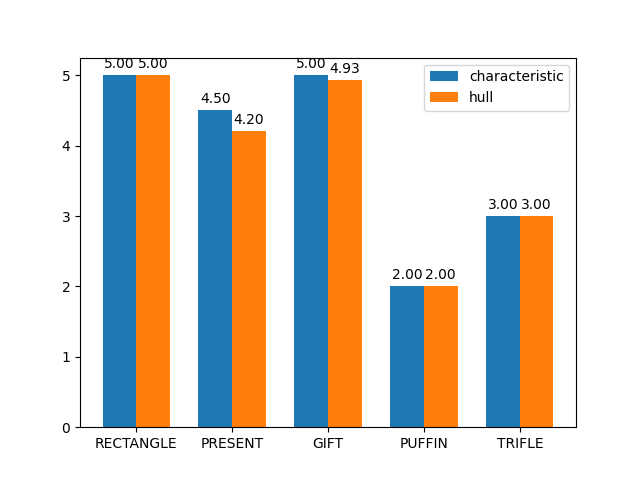
\includegraphics[width=1\textwidth]{fig/bar_ddt.png}
%	\label{fig:bar_ddt}
%\end{figure}

%\begin{figure}
%    \centering
%    \caption{Results on linear iterative distinguishers for some SPN block ciphers including KNOT-256, RECTANGLE, PRESENT, GIFT-64, PUFFIN and TRIFLE. The y-axis is the smallest negative logarithm of the linear correlation square of a linear iterative distinguisher. The height of a blue bar is the best average weight growth of a single linear iterative characteristic. The height of an orange bar is the best average weight growth of an $r$-round iterative linear hull with $r\leq 5$. The height of a green bar is is the best average weight growth of an $r$-round iterative linear hull with $r\leq 10$. }
%	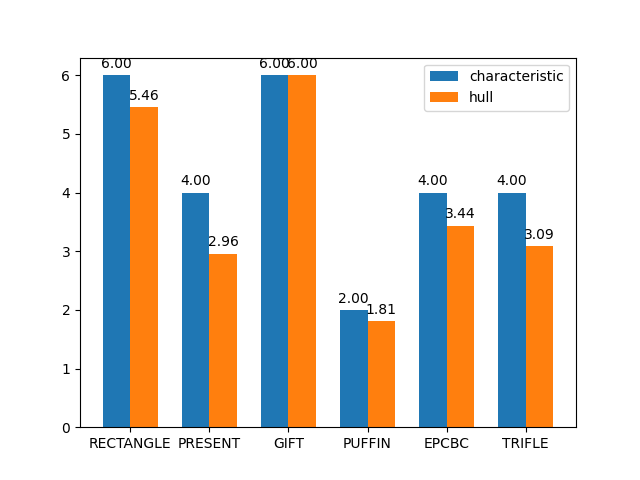
\includegraphics[width=1\textwidth]{fig/bar_lat2.png}
%	\label{fig:bar_lat2}
%\end{figure}

%In the following, we list the experimental settings and results for each of the ciphers. 
%Comparing the two figures, we find that linear iterative distinguishers have stronger clustering effect than differential ones. For each seperate primitives, we list the experimental settings and analysis of results. 

%\subsubsection{RECTANGLE \cite{zhang2015rectangle}} The state of RECTANGLE is treated in two dimensions. Each column is a 4-bit S-box which can be implemented using a bit-slice technique. Left rotational shifts are conducted on each of the 4 rows in parallel. The two operations of RECTANGLE has the rotational symmetry and thus we search for its rotational iterative characteristics. By setting $A=2$, the best differential rotational iterative characteristic we found is a 1-round one with input difference $x_0=0x2,x_5=0x6$, output difference $x_15=0x2,x_4=0x6$ and probability $2^{-5}$. By setting $A=3$, we can't find better rotational iterative differentials. By setting $A=2$, we found two best linear rotational iterative characteristics with average weight growth $6$. By setting $A=3$, the average weight growth of the best linear distinguisher we found is $5.46$ which is better than that obtained by only considering single linear characteristics. 

%\subsubsection{KNOT \cite{zhang2019knot}} KNOT is a round 2 candidate of the NIST lightweight cryptography standardization process. Its inner permutations are inheritors of RECTANGLE, also utilizing components with rotational symmetry. The primary version of it uses a 256-bit inner permutation. By setting $A=2$, we find its best differential and linear iterative characteristics. By setting $A=3$, we find stronger iterative distinguishers. 

%We set $A=3$ in both cases of differential and linear cryptanalysis. We find that the linear characteristics has clustering effect. But we note that the weight growth of the best iterative differential and linear distinguishers are equal, implying that its securities against differential and linear cryptanalysis are balanced. 

\subsubsection{PRESENT} The only best differential characteristic we find is exactly the one given in \cite{wang2008differential}. In \cite{ohkuma2009weak}, the author gives the construction of 1-bit linear characteristics. Our results are in compliance with the work in \cite{ohkuma2009weak} that the 1-bit linear characteristics have strong clustering effect. Note that the 1-S-box linear characteristics are 1-bit linear characteristic due to that the bit permutation spread the 4 output bits of 1 S-box to 4 input bits of 4 different S-boxes in the next round. 

\subsubsection{GIFT-64} From Table \ref{tab:ite-lat2}, it's shown that all primitives have clustering effect on linear characteristics except GIFT-64. To explore the reason, we draw the graph containing linear iterative characteristics in Figure \ref{fig:graph-gift64-lat2}. It's shown that the four iterative characteristics have no common masks. 

%\subsubsection{PUFFIN \cite{cheng2008puffin}} We set $A=1$ to find its best iterative characteristic. It has both comparatively weak securities against differential and linear cryptanalysis.

%\subsubsection{EPCBC \cite{yap2011epcbc}} We set $A=1$ in the linear case. We can't find any iterative differential characteristic though $A$ is set up to 3. But it has comparatively weak security against linear cryptanalysis. 

\subsubsection{TRIFLE} In \cite{liu2019iterative}, a 1-round differential characteristic is found using MILP method. It's also found using our method. Another best differential iterative characteristic we find has 127 rounds. 

\subsubsection{GIFT-128 \cite{banik2017gift}} We test out method on GIFT-128. We find no differential and linear characteristics even though $A$ is set up to 3. It's interesting that how to design a primitive with no low-weight iterative characteristic using a bit permutation as its linear layer. 

\subsubsection{ASCON \cite{dobraunig2016ascon}} We also test our method on the inner permutation of ASCON. We find no differential and linear characteristics even though $A$ is set up to 3. 
%attributed to its strong diffusion linear layer. 

%\begin{figure}\label{fig:plot_ite}
%    \centering
%    \caption{Results on some SPN block ciphers, which are RECTANGLE, PRESENT, GIFT64, PUFFIN, EPCBC and TRIFLE from top to bottom resp. For each subfigure, the x-axis is the number of rounds. For a subfigure in the left column, the y-axis is the weight of differential probability, while for a subfigure in the right column, the y-axis is the weight of correlation square. The red spot denotes the best single iterative characteristic with fewest rounds obtained by Algo. \ref{algo:find_ite_c_G}. The yellow (green, blue) line denotes the best iterative hull with $A=$1 (2, 3).} 
%	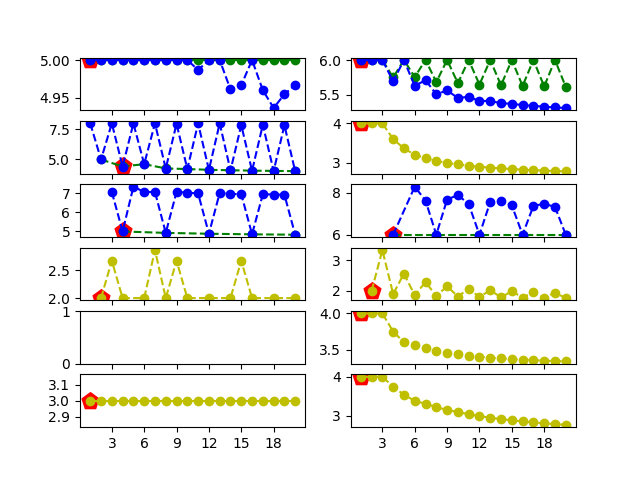
\includegraphics[width=1\textwidth]{fig/iterative.png}
%\end{figure}


\begin{figure}[htbp]
	\centering
	\caption{The generated graphs for RECTANGLE and KNOT256.}
	\subfigure[RECTANGLE, differential, $A=2$]{
	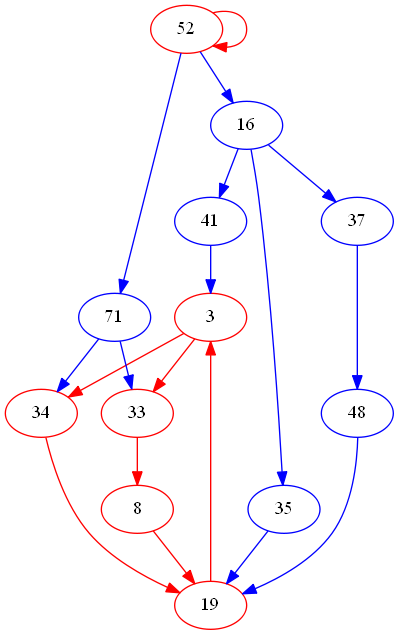
\includegraphics[width=5.5cm]{fig/graph_rect_ddt.png}
	\label{fig:graph-rect-ddt}
	}
	\quad
	\subfigure[RECTANGLE, linear, $A=2$]{
	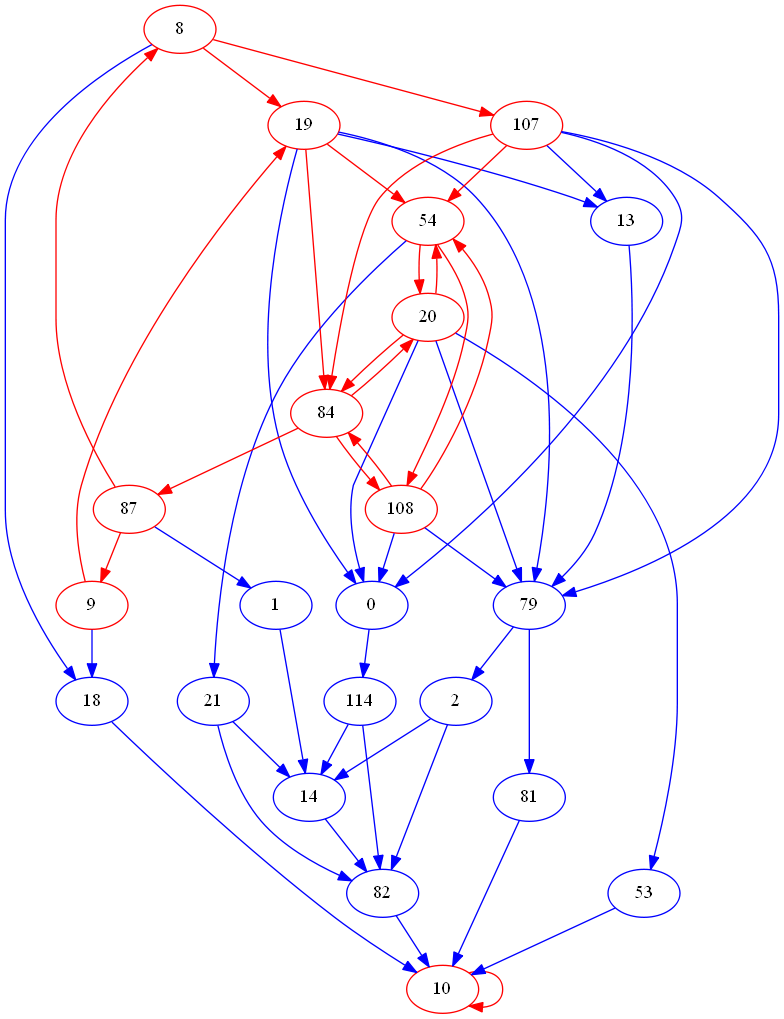
\includegraphics[width=5.5cm]{fig/graph_rect_lat2.png}
	\label{fig:graph-rect-lat2}
	}
	\quad
	\subfigure[KNOT256, differential, $A=2$]{
	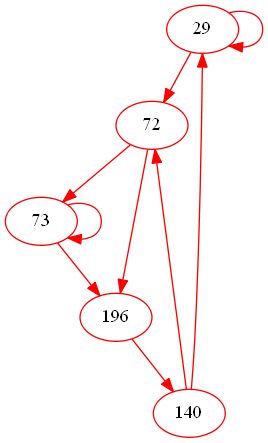
\includegraphics[width=4.5cm]{fig/graph_knot256_ddt.png}
	\label{fig:graph-knot256-ddt}
	}
	\quad
	\subfigure[KNOT256, linear, $A=2$]{
	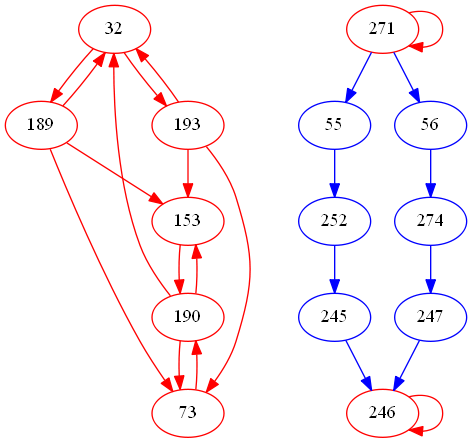
\includegraphics[width=6.5cm]{fig/graph_knot256_lat2.png}
	\label{fig:graph-knot256-lat2}
	}
\end{figure}

\begin{figure}
    \centering
	\caption{The generated graph containing linear iteractive characteristics for GIFT-64 when $A=2$}
	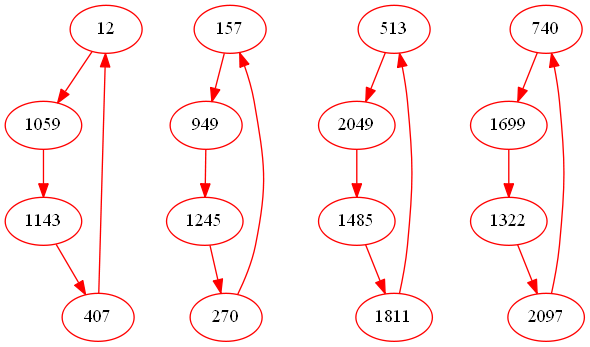
\includegraphics[width=0.8\textwidth]{fig/graph_gift64_lat2.png}
	\label{fig:graph-gift64-lat2}
\end{figure}

\subsection{Results on Finding the Best Differentials and Linear Hulls Containing Iterative Sub-characteristics}

We apply our Algorithm \ref{algo:msg}/\ref{algo:msg-equiv} to the 6 SPN primitives: KNOT-256, RECTANGLE, PRESENT, GIFT-64, PUFFIN and TRIFLE-BC. The results are given in Table \ref{tab:EDP} and Table \ref{tab:ELP}. 

For PRESENT, GIFT-64 and RECTANGLE, the results are very close to those in \cite{EPRINT:HalVej18}. For PUFFIN, we find both better differential and linear distinguishers than \cite{EPRINT:HalVej18} did. For TRIFLE-BC, the best differential distinguisher we find is a little better than the single 43-round differential characteristic given in \cite{liu2019iterative}. And we find a 51-round linear distinguisher while TRIFLE-BC has full rounds of 50. For KNOT-256, the designers only gave the results on the best single characteristics: a 48-round exploitable differential one and a 44-round exploitable linear one \cite{zhang2019knot}. We find a 53-round exploitable differential and a 56-round exploitable linear hull, improving the designers' results by 5 and 12 rounds respectively. 

\begin{table}
	\caption{Results on finding the best differential containing iterative sub-characteristics. $r$ is the number of rounds. $A$ is the maximum number of active S-boxes a difference we consider can has. $(rb,wb)$ determines the scope of extended differential characteristics we consider. $-\log_2\max\limits_{u\in S_0,v\in S_r}c(p_{u,v})$ is the probability of the best differential characteristic we find. $-\log_2\max\limits_{u\in S_0,v\in S_r}c(h^r_{u,v})$ is the probability of the best differential we find. $T$ is the running time of the whole process}\label{tab:EDP}
	\centering
	\begin{tabular}{|c|c|c|c|c|c|c|}
		\hline
		cipher & $r$ & $A$ & $(rb,wb)$ & $-\log_2\max\limits_{u\in S_0,v\in S_r}c(p_{u,v})$ & $-\log_2\max\limits_{u\in S_0,v\in S_r}c(h^r_{u,v})$ & $T$(h) \\
		\hline
		%PRESENT & 15 & 3 & (4,14) & 66 & 58.02 & 8s+5753s\\
		%PRESENT & 16 & 2 & (3,10) & 70 & 62.13 & 0s+42s\\
		PRESENT & 16 & 3 & (3,10) & 70 & 61.81 & 0.0 \\
		\hline
		%GIFT-64 & 12 & 2 & (3,13) & 58 & 56.57 & 0s+40s\\
		GIFT-64 & 13 & 2 & (3,13) & 62 & 60.42 & 0.0\\
		\hline 
		RECTANGLE & 14 & 2 & (6,25) & 61 & 60.65 & 133 \\
		\hline
		%KNOT-256 & 52 & 2 & (3,12) & 274 & 251.83 & 0s+10s\\
		%KNOT-256 & 52 & 2 & (3,10) & 274 & 252.41 & 1s+359s\\
		%KNOT-256 & 52 & 2 & (3,12) & 274 & 252.26 & 1s+1054s\\
		%KNOT-256 & 52 & 3 & (3,12) & 274 & 249.20 & 6s+11342s\\
		KNOT-256 & 53 & 3 & (3,12) & 274 & 254.38 & 0.2 \\
		\hline
		PUFFIN & 32 & 2 & (2,7) & 64 & 58.43 & 0.6 \\
		\hline
		TRIFLE-BC & 43 & 2 & (2,7) & 127 & 126.35 & 1.0 \\
		\hline
	\end{tabular}
\end{table}

\begin{table}
	\caption{Results on finding the best linear hull containing iterative sub-characteristics. $r$ is the number of rounds. $A$ is the maximum number of active S-boxes a mask we consider can has. $(rb,wb)$ determines the scope of extended linear characteristics we consider. $-\log_2\max\limits_{u\in S_0,v\in S_r}c(p_{u,v})$ is the correlation square of the best linear characteristic we find (correlation for KNOT-256). $-\log_2\max\limits_{u\in S_0,v\in S_r}c(h^r_{u,v})$ is the correlation potential of the best linear hull we find (correlation for KNOT-256). $T$ is the running time of the whole process}\label{tab:ELP}
	\centering
	\begin{tabular}{|c|c|c|c|c|c|c|}
		\hline
		cipher & $r$ & $A$ & $(rb,wb)$ & $-\log_2\max\limits_{u\in S_0,v\in S_r}c(p_{u,v})$ & $-\log_2\max\limits_{u\in S_0,v\in S_r}c(h^r_{u,v})$ & $T$(h) \\
		\hline
		PRESENT & 24 & 1 & (3,8) & 92 & 63.61 & 0.0 \\
		\hline
		GIFT-64 & 12 & 2 & (3,12) & 64 & 64.00 & 0.0 \\
		\hline 
		RECTANGLE & 14 & 3 & (3,14) & 68 & 62.31 & 1.5 \\
		\hline
		%KNOT-256 14 & 14 & 3 & (2,6) &  & 31.54 & 8s+\\
		%KNOT-256 24 & 28 & 3 & (2,6) &  & 63.20 & 8s+\\
		KNOT-256 & 56 & 3 & (2,6) & 161* & 125.83* & 75 \\%27
		%KNOT-256 & 56 & 3 & (2,6) & 161 & 125.262 & 27s+6.0h\\
		\hline
		PUFFIN & 32 & 2 & (4,14) & 64 & 50.70 & 0.0 \\
		\hline
		TRIFLE-BC & 51 & 1 & (2,7) & 200 & 126.58 & 0.0 \\
		\hline
	\end{tabular}
\end{table}

%\subsubsection{Comparison with the results in \cite{EPRINT:HalVej18}}

%We find that our results are very close to the results obtained in \cite{EPRINT:HalVej18}, which implies that the assumption that the best differential or linear distinguisher for an S-bP symmetric-key primitive is dominated by iterative characteristics is reasonable. 

\subsection{Results on differential and linear attacks against KNOT-AEAD and KNOT-Hash}

KNOT is a family of lightweight authenticated encryption algorithms and hash functions \cite{zhang2019knot}. The modes of operation of KNOT for AE and hash are shown in Figure \ref{fig:mode_aead},\ref{fig:mode_hash}. The modes are similar to the ones used in Ketje \cite{bertoni2014ketje} and ASCON \cite{dobraunig2016ascon}. The inner permutations are inheritors of RECTANGLE, which are bit-sliced lightweight. The round transformation has 3 steps: 4-bit S-boxes, row rotations and a constant addition. 

\begin{figure}
	\centering
	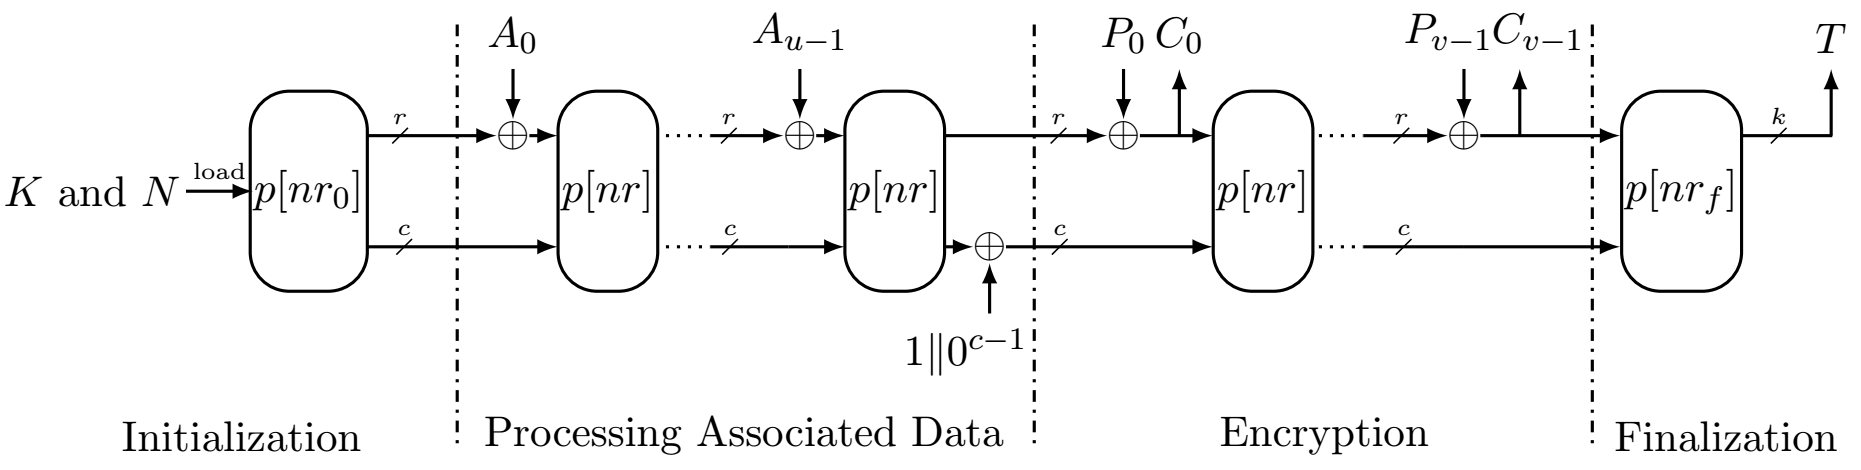
\includegraphics[width=1\textwidth]{fig/mode_aead.PNG}
	\caption{The operation mode of KNOT AEAD} \label{fig:mode_aead}
\end{figure}

\begin{figure}
	\centering
	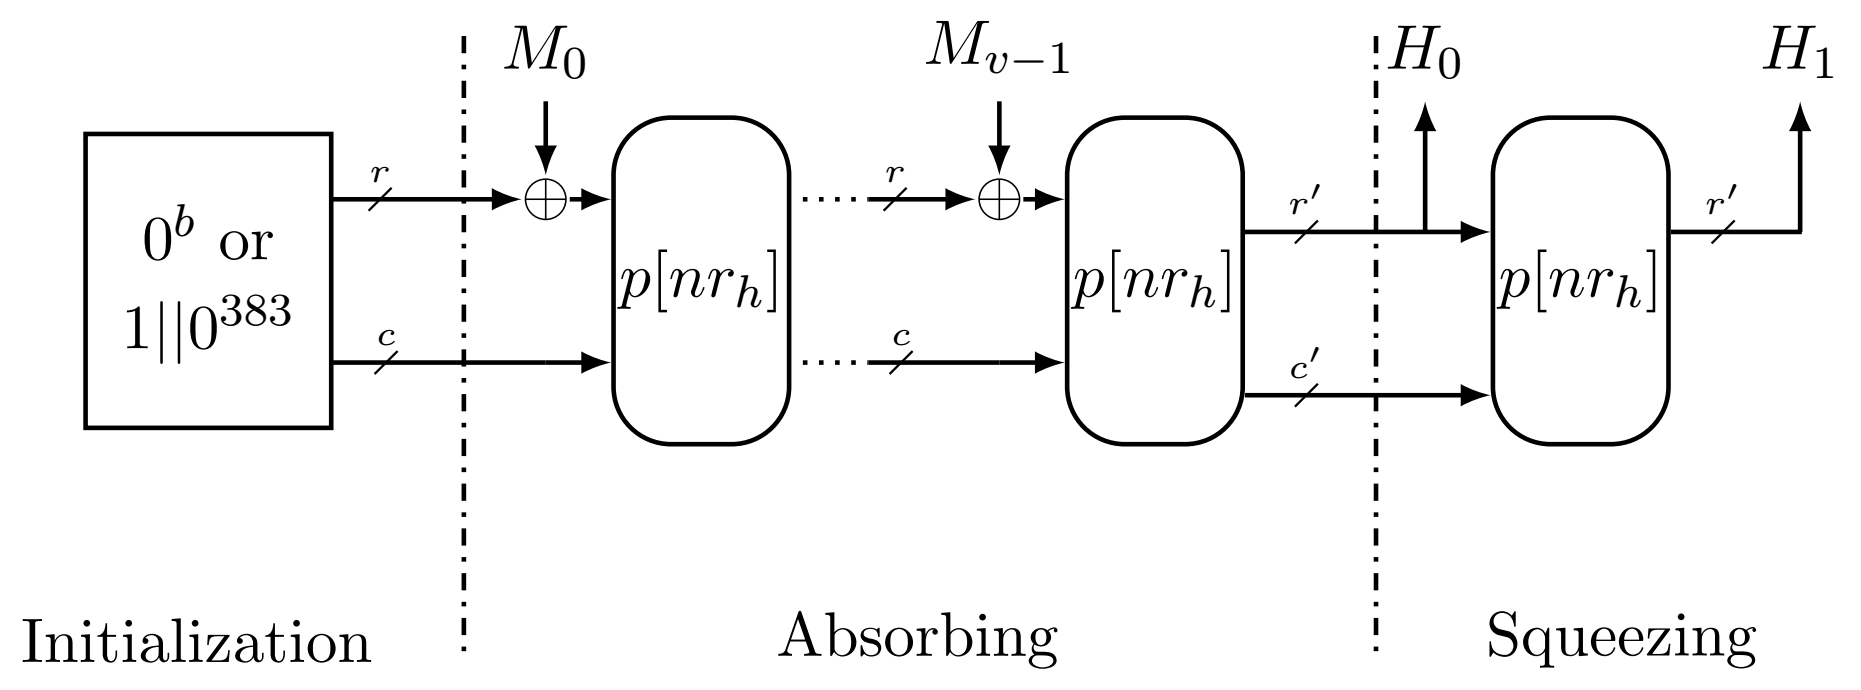
\includegraphics[width=0.7\textwidth]{fig/mode_hash.PNG}
	\caption{The operation mode of KNOT Hash} \label{fig:mode_hash}
\end{figure}

In the original specification document of KNOT, The largest differential probability and linear correlation is given. However, firstly, the differential and linear distinguishers with no restrictions can not be directly uesd to attack the MonkeyDuplex construction. Secondly, the clustering effect is not taken into consideration. Thirdly, because only the rate part and the tag part is visible, differences can be truncated in the capacity part and in the non-tag part. 

For the primary version of KNOT-AEAD, the block, rate, capacity, key and nonce size $b,r,c,k,n$ are $256,64,192,128,128$. For a inner state $S$, we can seperate it by the nonce and key part denoted by $(S_N,S_K),|S_N|=n,|S_K|=k$, by the rate and capacity part denoted by $(S_R,S_C),|S_R|=r,|S_C|=c$, by the tag and non-tag part denoted by $(S_T,S_{nT}),|S_T|=k,|S_{nT}|=b-k$.

For the primary version of KNOT-Hash, the block, rate, capacity and half-tag size $b,r,c,r'$ are $256,32,224,128$. For a inner state $S$, we can seperate it by the rate and capacity part denoted by $(S_R,S_C),|S_R|=r,|S_C|=c$, by the tag and non-tag part denoted by $(S_T,S_{nT}),|S_T|=r',|S_{nT}|=b-r'$.

In the following, we propose differential and linear attacks targeting different phases, each demanding specific restrictions on the distinguishers. The attacks proposed are general for cryptographic schemes based on MonkeyDuplex construction. For each attack, we give the largest differential probability or linear correlation of the longest distinguisher of the primary version of KNOT in Table \ref{tab:knot}.

\begin{itemize}
	\item \textbf{Diff-Init-D} This is a chosen-nonce differential distinguishing attack targeting the initialization phase of KNOT-AEAD. The input difference has the nonce part and key part $\Delta SI=(\Delta SI_N,\Delta SI_K)$. The output difference has the rate part and capacity part $\Delta SO=(\Delta SO_R,\Delta SO_C)$. We restrict that $\Delta SI_K=0$. And $\Delta SO_C$ is truncated. 
	\item \textbf{Linear-Init-KR} This is a known-nonce and known-plaintext linear key recovery attack targeting the initialization phase of KNOT-AEAD. The input mask $\Gamma SI=(\Gamma SI_N,\Gamma SI_K)$ and the output mask $\Gamma SO=(\Gamma SO_R,\Gamma SO_C)$. We restrict that $\Gamma SO_C=0$. Note that if for the best linear distinguisher $\Gamma SI_K\neq 0$, then the attack degrades to a distinguishing one, of which the probability is negligible. 
	\item \textbf{Linear-Enc-D} This is a known-plaintext linear distinguishing attack targeting the encryption phase of KNOT-AEAD. The input mask $\Gamma SI=(\Gamma SI_R,\Gamma SI_C)$ and the output mask $\Gamma SO=(\Gamma SO_R,\Gamma SO_C)$. We restrict that $\Gamma SI_C=0$ and $\Gamma SO_C=0$. 
	\item \textbf{Diff-Enc-F} This is a differential forgery attack targeting the encryption phase of KNOT-AEAD. The input difference $\Delta SI=(\Delta SI_R,\Delta SI_C)$ and the output difference $\Delta SO=(\Delta SO_R,\Delta SO_C)$. We restrict that $\Delta SI_C=0$ and $\Delta SO_C=0$. 
	\item \textbf{Diff-Final-F} This is a differential forgery attack targeting the finalization phase of KNOT-AEAD. The input difference $\Delta SI=(\Delta SI_R,\Delta SI_C)$ and the output difference $\Delta SO=(\Delta SO_T,\Delta SO_{nT})$. We restrictions that $\Delta SI_C=0$. And $\Delta SO_{nT}$ is truncated. 
	\item \textbf{Diff-Col-I} This is a differential collsion attack targeting the absorb phase of KNOT-Hash. The input difference $\Delta SI=(\Delta SI_R,\Delta SI_C)$ and the output difference $\Delta SO=(\Delta SO_R,\Delta SO_C)$. We restrictions that $\Delta SI_C=0$ and $\Delta SO_C=0$. 
	\item \textbf{Diff-Col-II} This is a differential collsion attack targeting the squeezing phase of KNOT-Hash. The input difference $\Delta SI=(\Delta SI_R,\Delta SI_C)$ and the output difference $\Delta SO=(\Delta SO_{T},\Delta SO_{nT})$. We restrict that $\Delta SI_C=0$ and $\Delta SI_{T}=0$. And $\Delta SI_{nT}$ is truncated. 
\end{itemize}

\begin{table}
	\caption{Results on the best differential and linear distinguishers for the primary version of KNOT}\label{tab:knot}
	\centering
	\begin{tabular}{|c|c|c|c|c|c|c|c|}
		\hline
		Attack Model & $r$ & $A$ & $(rb,wb)$ & $-\log_2\bbP$ or $-\log_2\Cor$\\
		\hline
		Diff-Init-D & 14 & 2 & (5,20) & 62.2 \\
		%Linear-Init-KR & 13 & 3 & (3,8) & 30.7*2=61.4 \\
		Linear-Init-KR & 13 & 3 & (3,8) & 31.3 \\%31.28
		%Linear-Enc-D & 12 & 3 & (3,10) & 30.2*2=60.4 \\
		%Linear-Enc-D & 12 & 3 & (3,8) & 30.44 \\
		Linear-Enc-D & 12 & 3 & (3,10) & 30.5 \\%30.52
		Diff-Enc-F & 12 & 2 & (5,20) & 62.4 \\
		Diff-Final-F & 13 & 2 & (5,20) & 61.4 \\
		Diff-Col-I & 12 & 2 & (5,20) & 62.7 \\
		Diff-Col-II & 13 & 2 & (5,20) & 61.4 \\
		\hline
	\end{tabular}
\end{table}

According to Table \ref{tab:knot}, it's suggested that the rounds of the initialization, encryption and finalization phases of KNOT-AEAD should be more than 14, 12 and 13 and the rounds of the absorbing and squeezing phases of KNOT-Hash should be more than 12 and 13. 

\subsection{Comparison with the method of enumerating characteristics}

To verify our results, fixing the input and output differences (masks) as those obtained using our method, we use the MILP method to enumerate characteristics with their differential probabilities (correlation amplitudes) larger than a bound. We respectively check on a 10-round differential and a 10-round linear hull.

For the 10-round difference propagation with input difference $X[32]=0x1, X[49]=0x1$ and output difference $Y[39]=0x1, Y[63]=0x1$, we enumerate its differential characteristics with probabilities between $2^{-56}$ and $2^{-69}$. The number of characteristics grouped by the probabilities are shown in Table \ref{tab:num-diff}. The total weight of a differential w.r.t. the maximum weight of a differential characteristic in it is shown in Figure \ref{fig:plot10-ddt}. We find the line approaches a horizontal one. Thus we believe the probability of the differential is very close to $2^{-53.49}$. Using our method, the number of characteristics grouped by the probabilities are also shown in Table \ref{tab:num-diff}. The probability sum is $2^{-53.53}$, which is very close to that obtained by the MILP method. By Table \ref{tab:num-diff}, the 10-round differential is dominated by characteristics containing iterative sub-characteristics. 

%the differential probability obtained by our method is $2^{-53.7}$ while that obtained by the MILP method is $2^{53.5}$. 

For the 10-round linear propagation with input mask $X[0]=0x1, X[25]=0x1$ and output mask $Y[24]=0x1, Y[41]=0x1$, we enumerate its linear characteristics with correlation amplitudes between $2^{-30}$ and $2^{-40}$. The number of characteristics grouped by the correlation amplitudes are shown in Table \ref{tab:num-linear}. The total weight of a linear hull w.r.t. the maximum weight of a linear characteristic in it is shown in Figure \ref{fig:plot10-lat2}. We find the line approaches a horizontal one. Thus the correlation square sum of the linear hull is very close to $2^{-56.21}$. Using our method, the number of characteristics grouped by the correlation amplitude are also shown in Table \ref{tab:num-linear}. The correlation square sum is $2^{-56.30}$, which is very close to that obtained by the MILP method. By Table \ref{tab:num-linear}, the 10-round linear hull is dominated by characteristics containing iterative sub-characteristics. 
%the linear correlation amplitude obtained by our method is $2^{-26.4}$ while that obtained by the MILP method is $2^{-25.5}$. We list the number of characteristics considered in both methods in Table \ref{tab:num-linear}. Our method underestimates the correlation amplitude for some characteristics with correlation amplitudes no smaller than $2^{34}$ are missing. But it holds that the distinguisher is dominated by iterative characteristics. 

\begin{figure}[htbp]
	\centering
	\caption{The total weight of a differential or linear hull w.r.t. the maximum weight of a characteristic }
	\subfigure[differential]{
	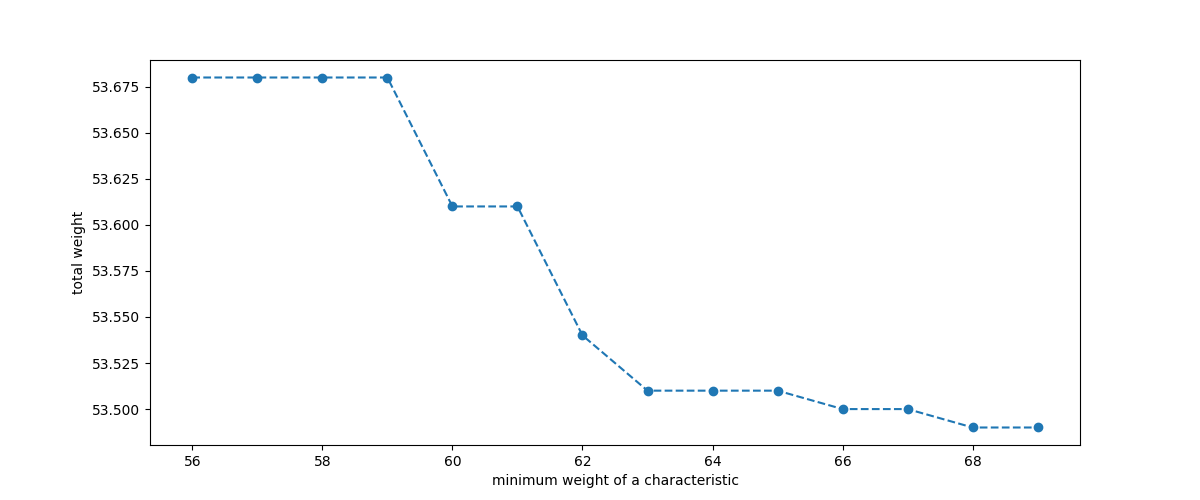
\includegraphics[width=9cm]{fig/plot10_ddt.png}
	\label{fig:plot10-ddt}
	}
	\quad
	\subfigure[linear]{
	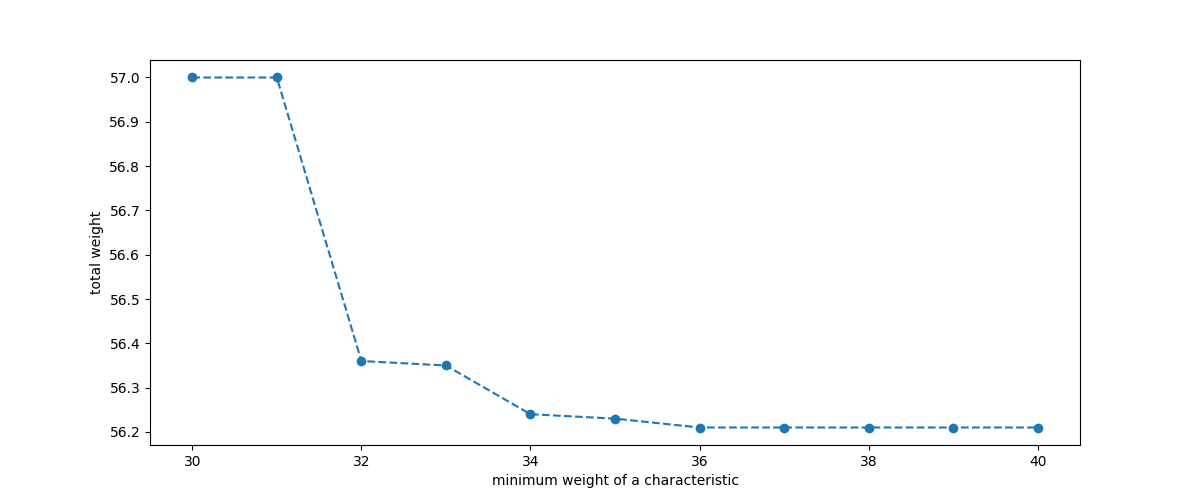
\includegraphics[width=9cm]{fig/plot10_lat2.png}
	\label{fig:plot10-lat2}
	}
	
\end{figure}

\begin{table}
	\caption{Results on the number of characteristics of the 10-round difference propagation grouped by the differential probabilities}\label{tab:num-diff}
	\centering
	\begin{tabular}{|c|c|c|c|c|c|c|c|c|c|c|c|c|c|c|}
		\hline
		$-\log_2|\Prob|$ & 56 & 57 & 58 & 59 & 60 & 61 & 62 & 63 & 64 & 65 & 66 & 67 & 68 & 69 \\
		\hline
		MILP & 5 & 0 & 0 & 0 & 4 & 0 & 17 & 12 & 0 & 12 & 36 & 1 & 38 & 59 \\
		\hline
		ours & 5 & 0 & 0 & 0 & 4 & 0 & 16 & 3 & 0 & 1 & 2 & 0 & 1 & 1\\
		\hline
	\end{tabular}
\end{table}

\begin{table}
	\caption{Results on the number of characteristics of the 10-round linear propagation grouped by the correlation amplitude}\label{tab:num-linear}
	\centering
	\begin{tabular}{|c|c|c|c|c|c|c|c|c|c|c|c|c|c|c|c|}
		\hline
		$-\log_2|\Cor|$ & 30 & 31 & 32 & 33 & 34 & 35 & 36 & 37 & 38 & 39 & 40 & 41 & 42 & 43 & 44\\
		\hline
		MILP & 8 & 0 & 72 & 4 & 264 & 72 & 648 & 364 & 1260 & 1092 & 2196 & - & - & - & - \\
		\hline
		%ours & 8 & 0 & 72 & 4 & 248 & 48 & 392 & 132 & 252 & 148 & 60 & 36 & 12 & 4\\
		ours & 8 & 0 & 64 & 0 & 224 & 8 & 480 & 56 & 736 & 160 & 752 & 216 & 584 & 216 & 224 \\
		\hline
	\end{tabular}
\end{table}




\section{Conclusion\label{sec:conclusion}}

In this work, we propose a new automatic tool searching for iterative trails for symmetric-key primitives based on S-boxes. We visualize the graph representation of iterative trails hoping to provide additional insignts. Based on the iterative trails, we efficiently estimate the probabilities of differentials and correlations of linear hulls. Our results show that the combination of iterative trails is very likely to enhance differential and linear propagations. What's more, our results show that, for ciphers we conduct experiments on with bit permutations as their linear layers, the good differentials and linear hulls are dominated by iterative trails. 

We have conducted an initial study on ASCON permutation. For its comparatively strong diffusion layer, iterative trails are difficult to be found. A question raised for designers is that, whether a cipher with bit permutation as its linear layer can have no iterative trails. And we plan to continue experimenting on ciphers with bit permutations as linear layers like ICEBERG, PUFFIN, etc. Ciphers with Feistel structure, like DES, are also going to be considered. 

In Algorithm \ref{algo:1}, we generate a graph describing the 1-round differential or linear propagations and then shrink it to a subgraph named as an iterative structure. The number of active S-boxes are limited. By using the technique in Section \ref{sec:expansion}, we can take more 1-round differential or linear propagations into consideration. The collection of interesting 1-round differential or linear propagations is heuristic. One may heuristically alter the way of the collection. 

In Algorithm \ref{algo:3}, we build a multistage graph by further considering trails extended from the vertices in the iterative structure. The weight of the trails are bounded in certain heuristic way. One can loose the bounds to obtain more accurate results but costing more time and memory. One can also heuristically alter the way how the bounds restrict the extension trails. 


%
% ---- Bibliography ----
%
% BibTeX users should specify bibliography style 'splncs04'.
% References will then be sorted and formatted in the correct style.
%
\bibliographystyle{splncs04}
\bibliography{mybibliography}
%
\begin{thebibliography}{8}
%\bibitem{ref_article1}
%Author, F.: Article title. Journal \textbf{2}(5), 99--110 (2016)

%\bibitem{ref_lncs1}
%Author, F., Author, S.: Title of a proceedings paper. In: Editor, F., Editor, S. (eds.) CONFERENCE 2016, LNCS, vol. 9999, pp. 1--13. Springer, Heidelberg (2016). \doi{10.10007/1234567890}

%\bibitem{ref_book1}
%Author, F., Author, S., Author, T.: Book title. 2nd edn. Publisher, Location (1999)

%\bibitem{ref_proc1}
%Author, A.-B.: Contribution title. In: 9th International Proceedings on Proceedings, pp. 1--2. Publisher, Location (2010)

%\bibitem{ref_url1}
%LNCS Homepage, \url{http://www.springer.com/lncs}. Last accessed 4 Oct 2017

%%%%%%%%%%%%%%%%%%%%%%%%%%%%%%%%%%%%%%%%%%%%%%%%%%%%%%%%%%%
%dedicated search:
%AKM97,BZL14,OMA95

%MILP search:
%MWG12,SHW14-1,SHW14-2,ZZDX19

%differential cryptanalysis:
%BS91,BS92

%linear cryptanalysis:
%M93,M94_1,M94_2

%ciphers
%Keccack:BDPV12,BDPVV14
%PRESENT:BKL07
%GIFT:BPP17
%Ascon:DEMS16
%AES:DR98,DR01,DR02
%RECTANGLE:ZBL15
%KNOT:ZDY19

%iterative trails
%K92,W08

%algorithms:
%J75,V03

%provable security
%R04
%%%%%%%%%%%%%%%%%%%%%%%%%%%%%%%%%%%%%%%%%%%%%%%%%%%%%%%%%%%

\bibitem{CXQ}
Yaxin Cui, Hong Xu, Wenfeng Qi. An Efficient method to construct Differential and Linear Characteristics of bit-slice block ciphers. (in Chinese). Journal of Cryptologic Research, 2020. Accepted. 

\end{thebibliography}
\appendix

\section{Visualization of Iterative Structures\label{app:visualization}}

\begin{figure}
	\centering
	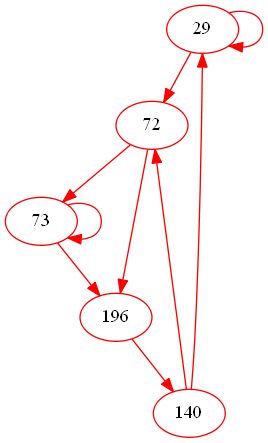
\includegraphics[width=0.7\textwidth]{fig/graph_knot256_ddt.PNG}
	\caption{the differential iterative structure $G^{IS}_{F,2}$ for KNOT-permutation-256} \label{fig:graph_knot256_ddt}
\end{figure}

\begin{figure}
	\centering
	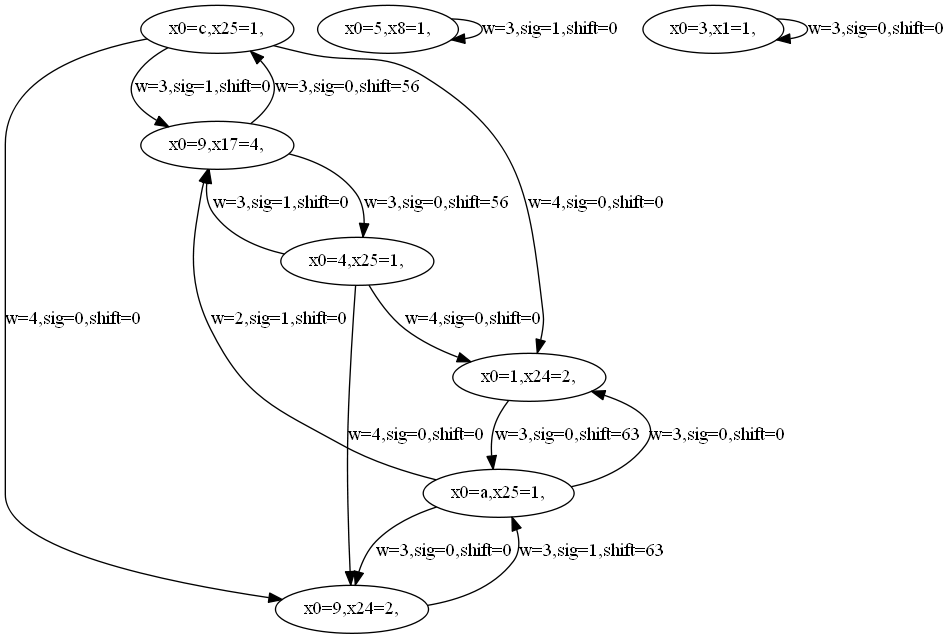
\includegraphics[width=0.7\textwidth]{fig/graph_knot256_lat.PNG}
	\caption{the linear iterative structure $G^{IS}_{F,2}$ of KNOT-permutation-256} \label{fig:graph_knot256_lat}
\end{figure}
\begin{figure}
	\centering
	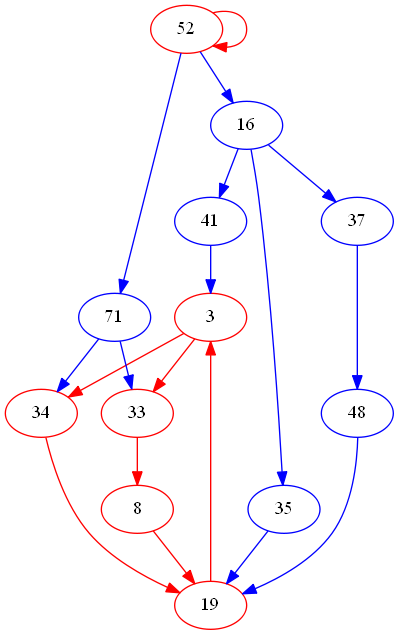
\includegraphics[width=0.7\textwidth]{fig/graph_rect_ddt.PNG}
	\caption{the differential iterative structure $G^{IS}_{F,2}$ of RECTANGLE} \label{fig:graph_rect_ddt}
\end{figure}

\begin{figure}
	\centering
	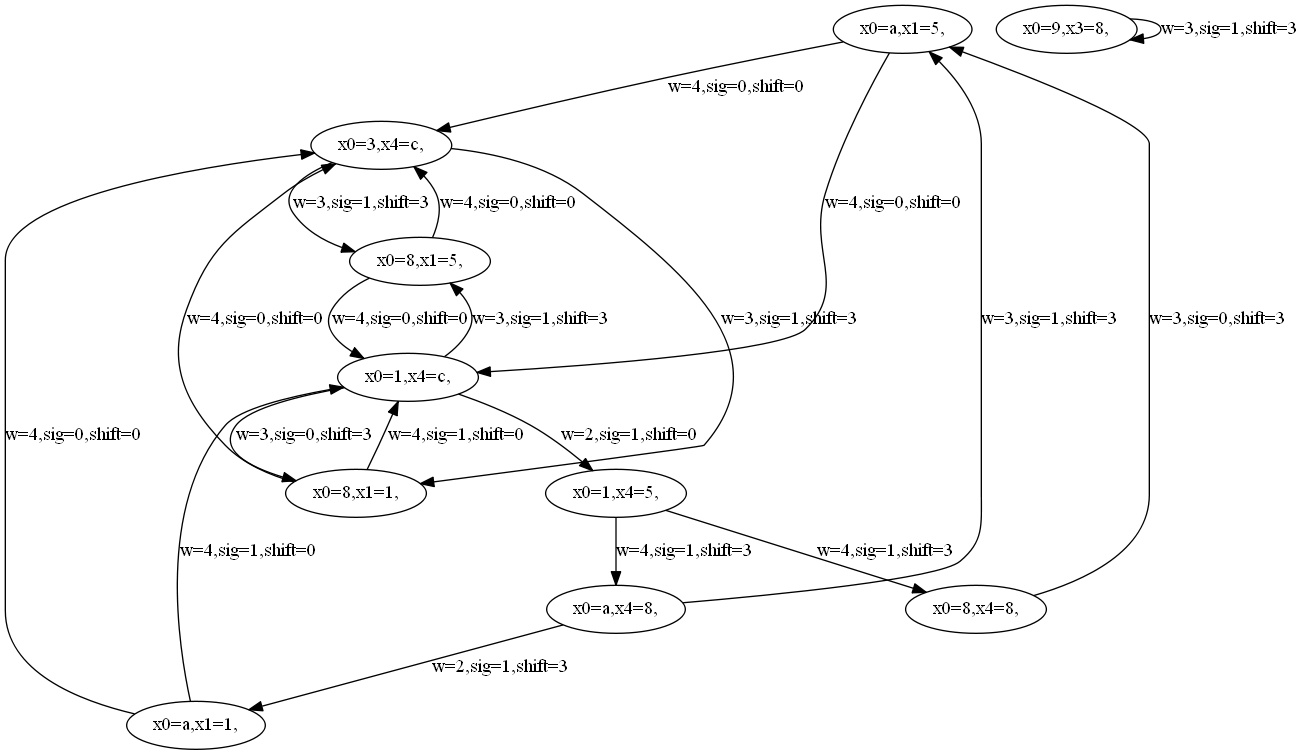
\includegraphics[width=0.7\textwidth]{fig/graph_rect_lat.PNG}
	\caption{the linear iterative structure $G^{IS}_{F,2}$ of RECTANGLE} \label{fig:graph_rect_lat}
\end{figure}

\begin{figure}
	\centering
	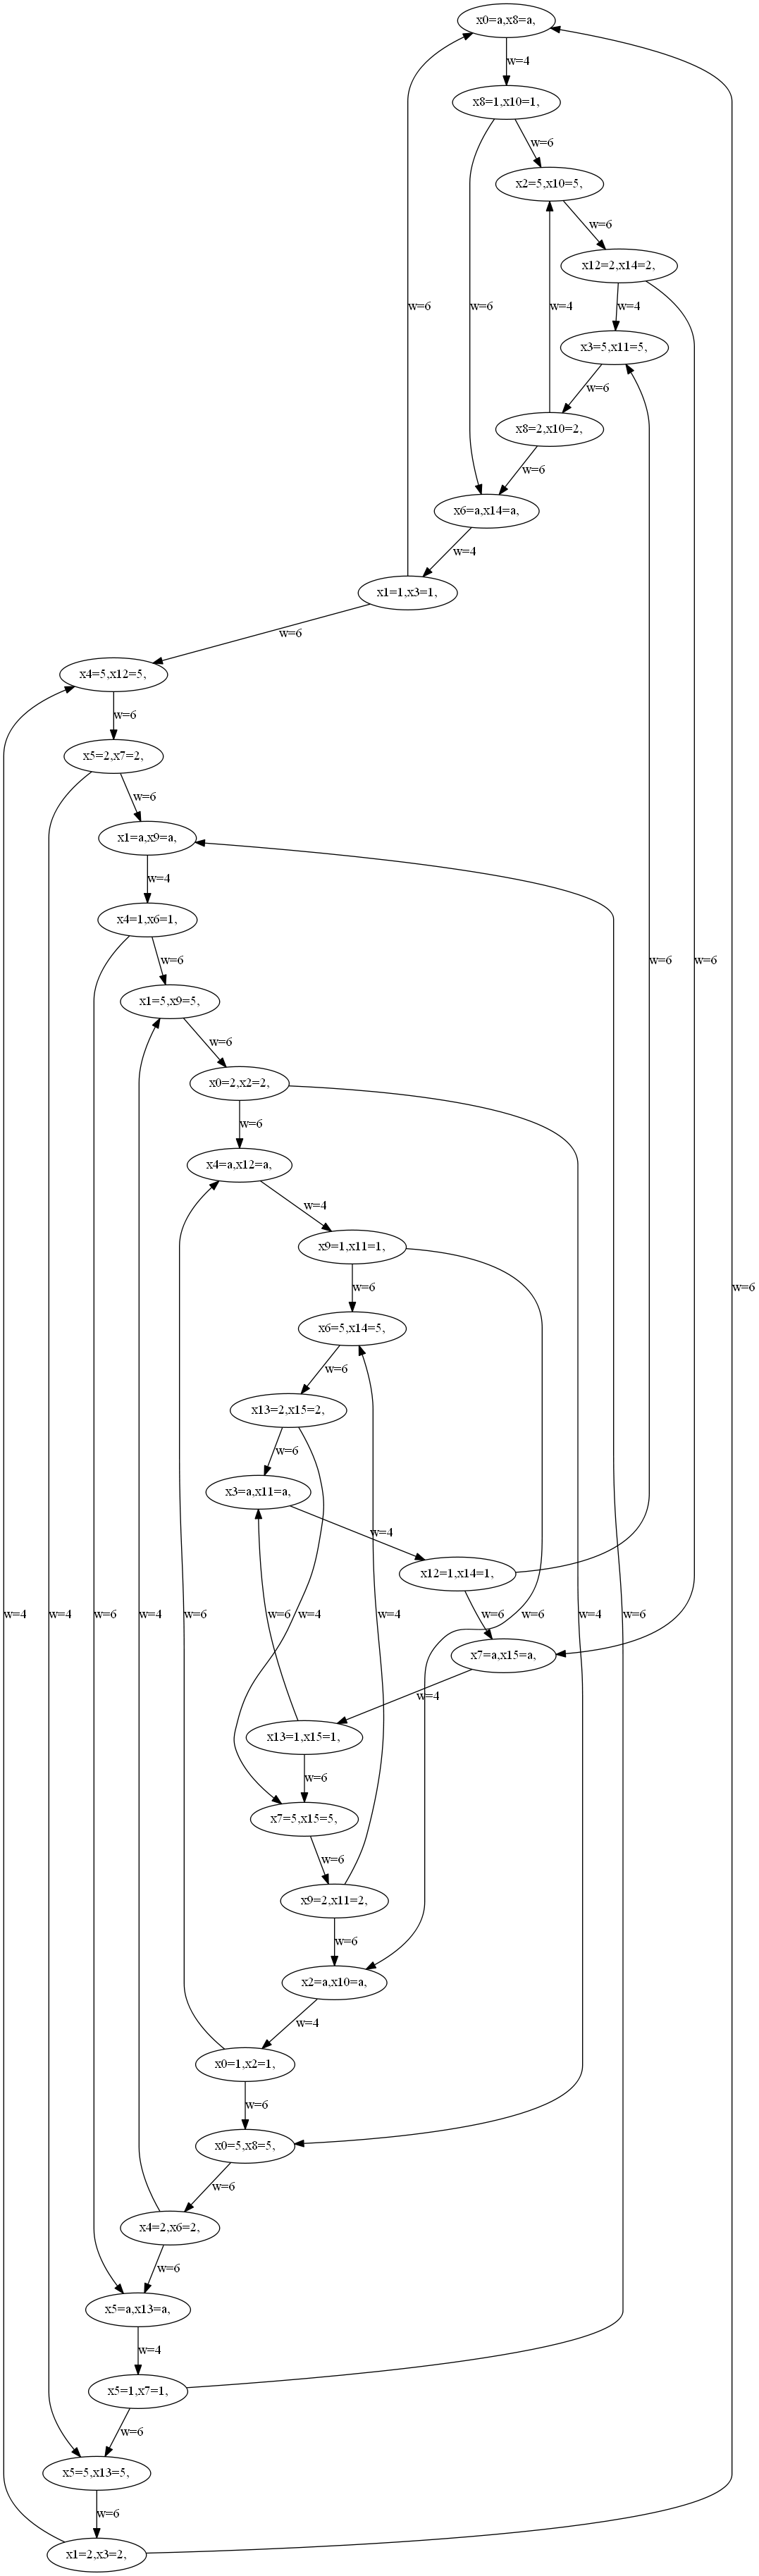
\includegraphics[width=0.4\textwidth]{fig/graph_gift_ddt.PNG}
	\caption{the differential iterative structure $G^{IS}_{F,2}$ of GIFT} \label{fig:graph_gift_ddt}
\end{figure}

\begin{figure}
	\centering
	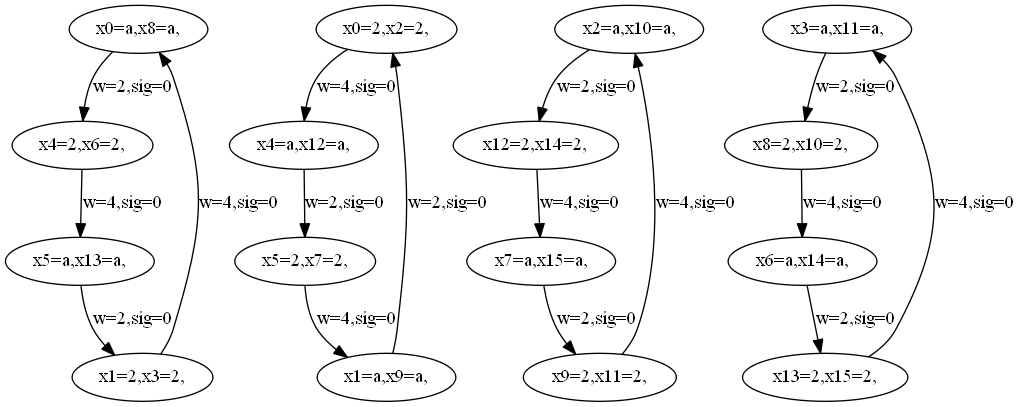
\includegraphics[width=0.7\textwidth]{fig/graph_gift_lat.PNG}
	\caption{the linear iterative structure $G^{IS}_{F,2}$ of GIFT} \label{fig:graph_gift_lat}
\end{figure}


\end{document}
